\documentclass[a4paper,twoside,12pt]{book}


\usepackage[italian]{babel}
\usepackage[latin1]{inputenc}
\usepackage[dvips]{epsfig}
\DeclareGraphicsExtensions{.ps,.eps}
\usepackage{subfigure}
\usepackage[T1]{fontenc}

\usepackage{fancyhdr}
\usepackage{amsmath}
\usepackage{amssymb}
\usepackage{a4}
\newcommand{\clearemptydoublepage}{\newpage{\pagestyle{empty}\cleardoublepage}}
\newcommand{\nohyphens}{\hyphenpenalty=10000\exhyphenpenalty=10000\relax}

%% Layout della pagina
%\pagestyle{fancyplain}
%\setlength{\headheight}{14.5pt}
%\addtolength{\headwidth}{\marginparsep}
%\addtolength{\headwidth}{\marginparwidth}
%\renewcommand{\chaptermark}[1]{\markboth{#1}{}}
%\renewcommand{\sectionmark}[1]{\markright{\thesection\  #1}}
%\lhead[\fancyplain{}{\bfseries\thepage}]%
%      {\fancyplain{}{\bfseries\rightmark}}
%\rhead[\fancyplain{}{\bfseries\leftmark}]%
%      {\fancyplain{}{\bfseries\thepage}}
%\cfoot{}

% Questa lunghezza rappresenta la lunghezza completa della pagine, compreso
% lo spazio per le note a margine
%\newlength{\fullpagelen}
%\setlength{\fullpagelen}{\textwidth}
%\addtolength{\fullpagelen}{\marginparsep}
%\addtolength{\fullpagelen}{\marginparwidth}

\makeatletter
\renewenvironment{thebibliography}[1]
  {%
    \chapter*{\bibname}%
    \addcontentsline{toc}{chapter}{\bibname}%
    \@mkboth{\MakeUppercase\bibname}{\MakeUppercase\bibname}%
    \list{\@biblabel{\@arabic\c@enumiv}}%
    {%
      \settowidth\labelwidth{\@biblabel{#1}}%
      \leftmargin\labelwidth
      \advance\leftmargin\labelsep
      \@openbib@code
      \usecounter{enumiv}%
      \let\p@enumiv\@empty
      \renewcommand\theenumiv{\@arabic\c@enumiv}%
    }%
    \sloppy
    \clubpenalty4000
    \@clubpenalty \clubpenalty
    \widowpenalty4000%
    \sfcode`\.\@m%
  }%
  {%
    \def\@noitemerr
    {\@latex@warning{Empty `thebibliography' environment}}%
    \endlist%
  }   % Finisce qui la ridefinizione di thebibliography

\makeatother


\newcommand{\name}{$\mathcal{H}$eaven } 
\newcommand{\namens}{$\mathcal{H}$eaven} 
\begin{document}


\pagestyle{fancy}
\renewcommand{\chaptermark}[1]{\markboth{#1}{}}
\renewcommand{\sectionmark}[1]{\markright{\thesection\ #1}}
\fancyhf{} \fancyhead[LE,RO]{\bfseries\thepage}
\fancyhead[LO]{\bfseries\rightmark}
\fancyhead[RE]{\bfseries\leftmark}
\renewcommand{\headrulewidth}{0.5pt}
\renewcommand{\footrulewidth}{0pt}
 \fancypagestyle{plain}{
\fancyhead{}
\renewcommand{\headrulewidth}{0pt}}


%\thispagestyle{empty} \vspace*{\stretch{1}} \hfill\begin{minipage}[t]{.618\linewidth}
\flushright\itshape Dedicata a chi vi pare :-) .
\end{minipage}
\vspace*{\stretch{3}}
 \clearemptydoublepage
%\chapter*{{\em Ringraziamenti}}

\emph{ Ringraziate chi vi pare...}
\clearemptydoublepage
%\thispagestyle{empty}
\chapter*{Prefazione}

Blablabla
\clearemptydoublepage
\tableofcontents \clearemptydoublepage

%\chapter{Executive Summary}
\section{Vedi Paper} \clearemptydoublepage
%\section{Semantic Web}
\section{Stream Processing}
\section{Stream Reasoning}
\section{Empirical Research}

Tichy and collaborators [15] evaluated 400 articles published in 1993, 50 of them randomly selected papers published by ACM in 1993 and the rest systematically selected from a few journals in Systems and Software Engineering, and classified the research re- ported in the paper in five categories (quoting [15] definitions): \begin{itemize}
\item Formal theory: articles whose main contributions are formally tractable propositions, e.g., lemmata and theorems and their proofs.
\item Design and modelling: systems, techniques, or models, whose claimed properties cannot be proven formally. Examples include software tools, performance prediction models, and complex hardware and software systems of all kinds. The papers in this class were further classified in the categories 0\%, 0–10\%, 10– 20\%, 20–50\, and +50\%, according to the proportion of the paper that was dedicated to the evaluation of the new system, technique, or model.
\item Empirical work: articles that collect, analyse, and interpret observations about known designs, systems, or models, or about abstract theories or subjects (as this paper does). The emphasis is on evaluation, not on new designs or models.
\item Hypothesis testing: articles that define hypotheses and describe experiments to test them.
\item Others: articles that do not fit any of the four categories above, e.g., surveys.
\end{itemize}

\section{Software Testing}
Software Testing (ST) techniques Starts with the intent of finding software bugs and ends with methods to evaluate system behaviour under testing conditions. In general software testing is an investigation over software products to evaluate the software quality. According to IEEE Standards  \cite{IEEEStd610.12-1990:glossary} there are two basic classes of software testing, black box testing and white box testing: 

\begin{itemize}
\item Black box testing [BBT] - it ignores the internal mechanisms of a system or component and focuses solely on the outputs
generated in response to selected inputs and execution conditions.
\item White box testing [WBT] - is takes into account the internal mechanism of a system or component. 
\end{itemize} 

Black-box testing  methods  examine the functionality of a system without peering into its internal structures or workings. BBT exploits test cases built around specifications and requirements of the software. An external descriptions of the software is mandatory, and it must also include software specifications, requirements and design parameters.  The test designer selects both valid and invalid inputs and determines the correct output without any knowledge of the test object's internal structure.

White-box testing  method instead exploits complete knowledge about software internal structures. In WBT an internal perspective of the system is required to design test cases. The test designer analyses the code, understand the expected output and chose input properly  to exercise paths he found. 

ST tries to offer an objective, independent view of the software, usually with Software Performance Testing, defined as  \textit{testing conducted to evaluate the compliance of a system or component with specified performance requirements} \cite{IEEEStd610.12-1990:glossary}. Once  the key transactions and their data requirements are identified, the test designer creates a number of different types of performance tests, in order to evaluate different software characteristics. The design of the test follows the researcher needs about which behaviour evaluate. The choice depends on the nature of the application and how much time is available for performance testing. The following testing terms are generally well known in the industry \cite{Molyneaux:2009:AAP:1550832}:

\begin{itemize}
\item \textit{Load testing} - it is the simplest form of performance testing, its aim is to understand the behaviour of the system under an expected load (the load kind depends on the software system) and meet performance targets for availability, concurrency or throughput, and response time. This test will give out the response times of all the critical transactions and it can point out bottlenecks in the application software. Load testing is the closest approximation of real application use.

\item \textit{Stress testing} -  it is used to understand the upper limits of capacity of a system and determine the system's robustness in terms of extreme load. A stress test may causes the application or some part of the supporting infrastructure to fail. The results of this kind of test are  capacity measure as much as performance. It's important to understand software limitations, in order to face future growth of application traffic, which may be hard to predict.

\item \textit{ Soak testing} - it is performed to determine if the system can sustain the continuous expected load. It essentially involves applying a significant load to a system for an significant period of time. The goal is to discover how the system behaves under sustained use or identify steady state conditions. During soak tests, memory utilization is monitored to detect potential leaks. Also important, but often overlooked is performance degradation, i.e. to ensure that the throughput and/or response times after some long period of sustained activity are as good as or better than at the beginning of the test. 
\end{itemize} 

\section{Benchmarks}
A benchmark is a procedure, problem, or test that can be used to compare systems or components to each other or to a standard \cite{IEEEStd610.12-1990:glossary}. Benchmarking is the primary method for measuring the performance of a systems, hardware or an application[7]. Benchmark results are used to evaluate the performance of a given system on a well-defined workload \cite{Menasce:2001:CPW:560806}.

Many benchmark tests exists to evaluate a wide variety system or applications under under different types of workloads. The user groups like the Transaction Processing Performance Council (TPC) \footnote{http://www.tpc.org/information},  a non-profit corporation founded to define transaction processing and database benchmarks, or analogues corporations are useful resources of be informed about updated types of benchmarks. 

Generic benchmarks allows the quantitative comparison of system performances or price/cost. In database context performance is typically a throughput metric (work/second) and price is typically a five-year cost-of-ownership metric. The quantitative comparison requires the benchmark to be run on several different systems and to record each system is measurements.  The estimation evaluated from results is usually the relative system performance, because the cost of implementing and measuring a specific application on many different systems is almost always prohibitive.

\subsection{Domain Specifc Benchmarks}  \label{sec:tcp}

A single metric can not measure the performance relative to all application of a computer systems \cite{DBLP:books/mk/Gray93}. Performances depend striclty on the application domain, because each system is designed for a few problem in a domain and may be inadequate to perform other tasks.

It is worth to note the work of Jim Gray about Domain-specific benchmarks, a kind of benchmarking methods and tools  which responds to computer system diversity. A Domain-specific benchmark specifies a synthetic workload characterizing typical applications in that problem domain. 

In order to distinguish among several solution and workload, Gray states four key criteria that a Domain-Specific Benchmark must meet to be useful\cite{DBLP:books/mk/Gray93}. It must be:
\begin{itemize}
\item Relevant: It must measure the peak performance and price/performance of systems when performing typical operations within that problem domain.
\item Portable: It should be easy to implement the benchmark on many different systems and architectures.
Gray: Introduction 3
\item Scalable: The benchmark should apply to small and large computer systems. It should be possible to scale the benchmark up to larger systems, and to parallel computer systems as computer performance and architecture evolve.
\item Simple: The benchmark must be understandable, otherwise it will lack credibility.
\end{itemize} 


\subsection{Reasoning Benchmark}\label{sec:lubm}

The number of different reasoners available is increasing and many of them are already commercial solutions. Usually reasoner are able to process very expressive ontology languages, which can represent rather complete knowledge, however there is an high demand of  less expressive ontology languages, which are less expensive in term of reasoning or other computational tasks. Commercial reasoner tries to solve the issue called \textit{computational cliff}, they face the trade-off between \textit{complexity and expressiveness} versus \textit{scalability}. Benchmarking tools are useful to evaluate reasoning system w.r.t. ontology languages.
\cite{bock2008benchmarking} The most important Benchmark suite is the Lehigh University Benchmark  (LUBM) \cite{Guo2005}. This work proposes a  method for benchmarking Semantic Web knowledge base systems and provide an example of such a benchmarks.

Reasoning benchmarking environment requires:
\begin{itemize}
\item Ontology: LUBM exploits a synthetic ontology named Univ-Bench\footnote{http://www.lehigh.edu/~zhp2/2004/0401/univ-bench.owl} ,which describes universities, departments and the activities that occur at them. However, the popularity of OWL is high and that
many more ontologies are now available, and recent automated benchmarking tools allow testing performance with such ontologies\cite{gardiner2006automated}.

\item Workload:LUBM provides an random data generator, called UBA (Univ-Bench Artificial data generator), which creates extensional data over the Univ-Bench ontology. \cite{Guo2005}

\item Queries: LUBM comes with fourteen test queries to test the reasoning capabilities over the workload. LUBM method contains criteria for query definition which consider for example \textit{Input size} or \textit{Complexity} to stress the reasoner and evaluate performances.
\end{itemize}

Finally, Reasoning benchmarking require to understand which metrics evaluate such a system\cite{Guo2005}. LUBM contains three metrics which are commonly used in other database benchmarks.\begin{itemize}
\item \textit{Load Time,the stand alone elapsed time for storing the specified dataset to the system};
\item \textit{Repository Size, the resulting size of the repository after loading the specified benchmark data into the system};
\item \textit{Query Response Time}, as in databases benchmarking, for each test query the evaluation consist in:
  	1) Open the repository; 2) Execute the query for 10 times and compute the average response time. 3) Close the repository
\end{itemize}

LUBM contains also two specific reasoning metrics: \textit{Query Completeness and Soundness}: partial answering is possible in semantic web, indeed LUBM evaluate the \textit{degree of completeness of each query answer as the percentage of the entailed answers that are returned by the system is also evaluated}. Moreover, LUBM also provides a metric for measuring the combination of  query response time and answer completeness and soundness, to  appreciate the potential trade-off.

\subsection{SDMS \& CEP Benchmarking}\label{sec:linear-road}

Initial work on Streaming data like Linear Road \cite{arasu2004linear} firstly poses  several challenges to the design of a benchmark.  Moreover, the variety of CEP and SDMS domains and the lack of standards in query languages and data formats extends these benchmark design challenges. First of all SDMS Benchmarking must consider the challenges presented in the Linear Road work:
\begin{itemize}
\item  \textit{Semantically Valid Input} -  Input data can not be randomized but should have some semantic validity.
\item  \textit{Continuous Query Performance Metrics} - Standard DBMS time to completion metrics is inadequate. Query Response Time and Supported Query Load 
\item  \textit{Results Correctness} - benchmark implementations must be validated w.r.t the queries, which influence the results, to ensure that results are consistent with the benchmark specifications 
\item  \textit{Query Language Independence}: no standard query language for streaming systemsn exist, thus the query requirements must be language independent
\end{itemize}

Linear Road meets all the challenges above by design. The benchmark consist into a simulation of  an urban freeway system where toll charges are dynamically determined. The Input data contains a stream of position reports, which specify the location of a vehicle every 30 seconds, and historical query requests, which may be issued by a vehicle with some fixed probability every time it emits a position report.

Further works, like the BiCEP project\footnote{http://bicep.dei.uc.pt} try to identify some o requirements for CEP benchmarking and develop a synthetic benchmarking set to measure the event processing activity such systems. CEP Benchmarking are evaluated with Jim Gray criteria presented in Section \ref{sec:tcp}. 

\begin{figure}[tbh]
  \centering
	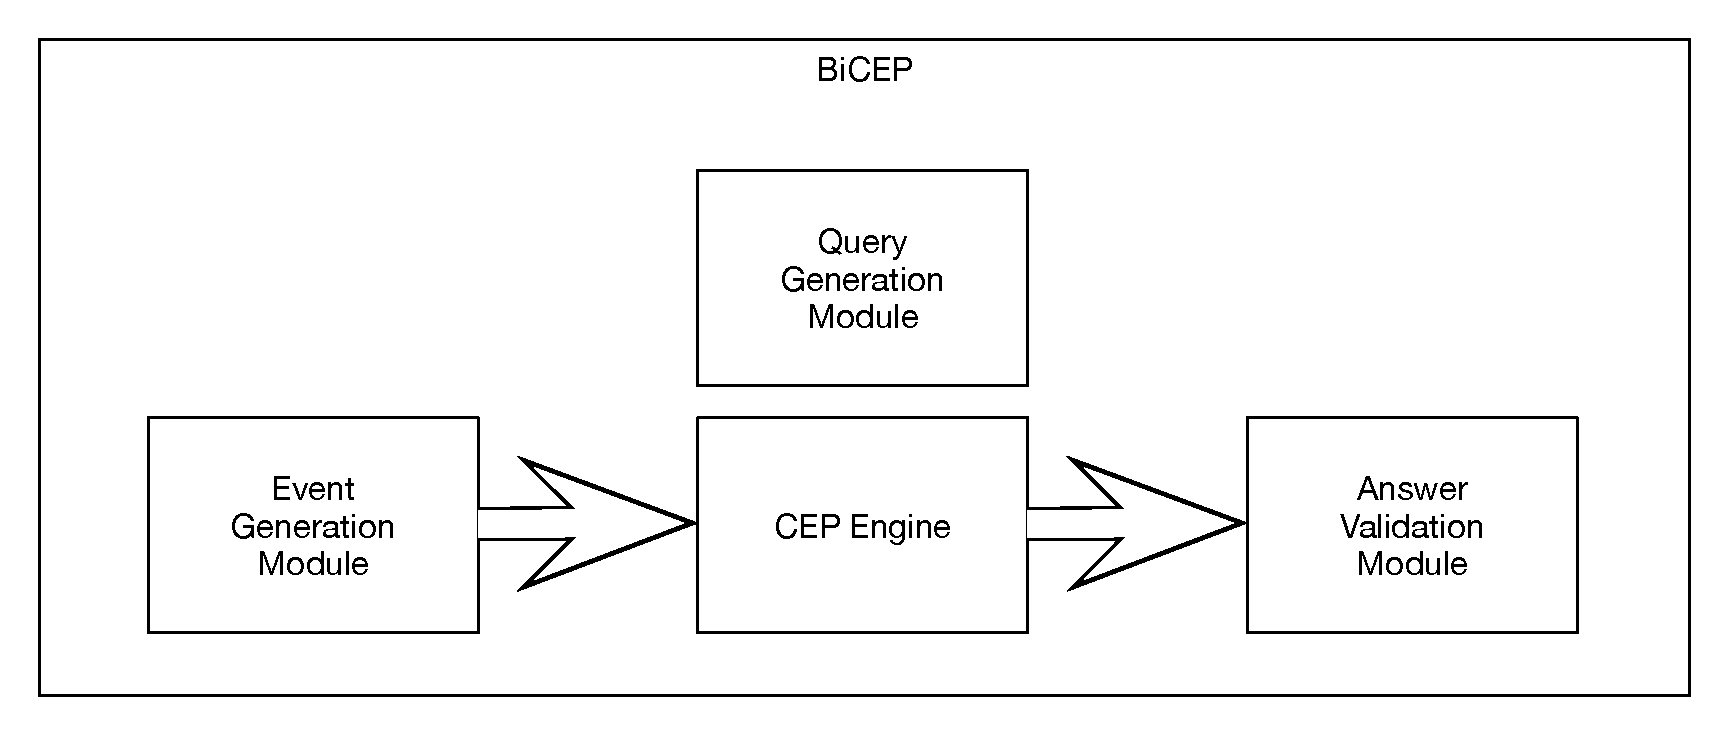
\includegraphics[width=\linewidth]{images/bicep_schema}
	\caption{BiCEP system  modules and the CEP engine} 
  	\label{fig:bicep-schema}
\end{figure}

BiCEP project also presents an first schema model for a benchmarking system, reported in Figure \ref{fig:bicep-schema}. The BiCEP benchmarking system will produce all the input trough the Event Generator Module, and consume the result output from the BiCEP CEP engine, with the Answer Validation Module. The Figure above also show how the CEP engine in interfaced with BiCEP modules, in order to ensure that any buffering, event cleaning or event transformation phase that happens at the CEP engine is part of the overall performance measure. Synthetic benchmarks offers many benefits like data availability, experimental control, and scalability. However, it is is hard to develop a synthetic benchmark that is representative of such a wide range of CEP applications and at the same time. BiCEP development is oriented towards a set of small domain specific synthetic benchmarks with different data sets and different queries \cite{bizarro:DSP:2007:1143}.

Finally, BiCEP project presents a set of metrics for CEP benchmarking, the most relevant ones in performance evaluation context are: \textit{Response time}: the time since the last event of some event pattern is fed into the system until the system notifies the event pattern detection. \textit{Scalability} in order to compare system with different scale levels; \textit{Adaptivity} the system response to input variation is mandatory, because CEP system rarely face stable input streams that allow the CEP engine to reach a steady state condition.



\subsection{Stream Reasoning Benchmark}
%\subsubsection{SRBench}
SRBench [5] proposes a suite of test queries and defines metrics to evaluate the
performance of the system. This benchmark contains 17 queries to gather the
properties of the RDF stream engines. The queries vary to ensure that several
features of the target system are tested: queries involving single or multiple input
streams, queries over stream-only data sources or over mixed stream and static
data source, etc. In [5] the authors applied the benchmark on the existent RDF
stream engines, and explained the differences in term of supported functionalities.
Time and memory performance tests, and scalability tests are not targeted
in the actual version of SRBench.
%\subsubsection{LSBench}
LSBench [6] proposes three tests to evaluate the RDF stream engines. The
first one is a functional test to verify the operators and the functionalities supported
by the engines: it is a test similar to the one proposed by SRBench. The
second test is a correctness test: its goal is to verify if the tested RDF stream
engine produces the correct output. Actually this analyses only the number of
produced answers, assuming that the contents of the output are correct. Finally,
the third test is a maximum input throughput test: it has the goal evaluate the
maximum throughput of the RDF stream engines. This test is done increasing
the rate of data in the stream and verifying the number of the answers. For each
test a set of 12 queries is provided; similarly to SRBench, the queries vary to
take into account different features of the engines (single and multiple streams,
presence of static data, etc)

%\subsubsection{Correttezza}
%\subsubsection{Seven Commandaments}

 \clearemptydoublepage
\chapter{Problem Settings}

In this chapter we present firstly the question that leads our research and the motivations which sustain it. Next we extend in Section x  the requirements posed by the research question and the issues it involves. In the end we provide the technical formalization of those requirements and why our work must cover them, which issue they solves and which limitation we have to face to.

\section{Overview}
Stream Reasoning research filed wonders to achieve a tight integration of known reasoning systems and DSMS, to exploit reasoning techniques upon rapid changing information \cite{Background SW, DSMS, SR}. An RDF Stream Processing Engine, shortly RSP Engine, is the abstraction that realizes this integration: it can  manage rapidly changing worlds at the semantic level and answer complex queries typical of Semantic Web. The Stream Reasoning community is working on the standardization of a protocol to talk with RSP Engines, which actually can be implemented applying a number of RSP techniques. Their number is increasing together with the need of shared practices and tools to perform analyses and evaluations. As stated in Chapter 2, benchmarking RSP Engines is possible thanks to the proposed RDF streams, continuous queries, and performance measurements. The critics on these works have showed their limits and further developments partially went beyond \cite{paper paper}. However, the the community still lacks the formalization of a comparative approach and an infrastructure that allows to apply it rigorously.

In this thesis we propose \namens, a framework that tries to solve the Stream Reasoning need of a Systematic Comparative Approach on RSP Engine evaluation.



\section{Requirements} \label{sec:requirements}

We developed \name in order to simplify and support Systematic Comparative Research Approach on RSP engines. To this extent we need to answer the following questions: 
\begin{enumerate}
\item[Q.1] How can the behaviour of system be evaluated? 
\item[Q.2] What makes this evaluation rigorous? 
\item[Q.3] How can this rigorous evaluation be automated?
\end{enumerate}

A proper answer to Question Q.1 can be stated exploiting the traditional definition of \textit{experiment}: a test under controlled conditions that is made to demonstrate a known truth or examine the validity of an hypothesis. Going deeply, we answer Q.2 bringing about the notions of \textit{reproducibility}, \textit{repeatability}, and \textit{comparability} of experiments. The concepts we identified make easy to answer Q.3 formalising the technical requirements for \namens.

Reproducibility is related to the variation in measurements made on a subject under changing conditions. The concept of experiment gather this conditions. \name must allow its users to define it in details: 
\begin{enumerate}
\item[R.1] it must be \textit{test data independent}, thus allowing users to chose relevant RDF data streams and ontologies from their domain of interest. %R.2.1
\item[R.2] it must be \textit{query independent}, thus allowing users to register relevant queries from their domains of interest. %R.2.2
\item[R.3] it must be \textit{engine independent}, thus allowing users to put an RSP engine on the test stand by the means of easy to implement software interfaces, e.g., it should adopt an event-base architecture as normally done by RSP engines and present events to RSP engine in a simple to parse RDF serialisation. %R4 e R5
\item[R.4] it must include a \textit{basic set of performance measurements} \cite{DBLP:conf/esws/ScharrenbachUMVB13} including \textbf{Latency} -- defined as the delay between the injection of an event in the RSP engine and its response to it --, \textbf{Memory Usage} -- defined as the difference between total system memory and free memory --, and \textbf{Completeness \& Soundness} of query-answering results.  %R2.3
\item[R.5] it should enable users to extend the test stand adding their own software sensors in order to other performance measurements %???
\end{enumerate}

In terms of software engineering the list of requirements above demands an \textit{Extendable Design} [R6], i.e.,  the possibility to replace theoretically each module with one with the same interfaces, but different behaviour, without affecting architecture stability.

Repeatability of measurements regards the variation in repeat measurements made on the same subject under identical conditions. \name must not affect the RSP engine evaluation to grant it. This from a practical point of view poses two requirements to the test stand:
\begin{enumerate}
\item[R.7] it must not be running when the RSP engine is under execution. %R.1.2
\item[R.8] it must have reduced (and possibly constant) memory footprint. %R.1.1
\end{enumerate}

The comparative research is case-oriented. It allows the systematic analysis of complex cases, exploiting comparable metrics. The complex cases are seen as configurations, a combination of known properties, upon which is possible to identify parallelism or state contrasts. A Systematic Comparative Research Approach (SCRA) requires firstly the definition of \textit{Metrics that allow comparison} and standardization of \textit{Evaluation conditions}.  \name must support the collection of the performance measurements as custom metrics [R.9]; again the concept of experiment is required a formalization for the execution setting. The next step consists in providing \textit{Tools for qualitative analysis}, which allow visualisation of the results [R.10].

Last but not least, to simplify SCRA is important to identify \textit{Simple terms of comparison}, which have an experimental validity. \name contains specific modules to fulfil this requests, more details about them in Chapter 6 . Those modules support the consequent need of \textit{Examples of successful analysis and evaluations}, which can be exploited as guidelines. Chapter 7 of this thesis present a set of experimental evaluations which show deeply the potential of \name. \clearemptydoublepage
%In this chapter we present  \namens,  an open source framework for Systematic Comparative Research on RSP Engine.
It consists in four baselines and two main components: the Test Stand and the Analyser. Firstly, Section \ref{sec:teststand} introduces the Test Stand, which satisfies requirements from R.1 to R.8 and from R.10 to R.12, by executing experiments on an RSP Engine. Section \ref{sec:baselines} describes the Baselines, four RSP Engines that are included in \name as naive terms of comparison, since they fulfil requirements R.13 and R.14. Finally, Section \ref{sec:analyser} presents the Analyser, which addresses requirements R.9 and R.10  allowing the user to visualise, investigate and compare experiment results. %Soundness and completes of the query answering process are assessed post-hoc by comparing the results of an RSP engine with a term of comparison whose results are correct (see Section 5).

\section{Test Stand}\label{sec:teststand}

Aerospace engineering defines an Engine Test Stand as a facility used to develop, study and characterise engines. It allows to test operating regimes and offers measurement of several variables associated with engine process. A Test Stand may uses actuators for attaining a specific engine state, which is a unique combination of the engine properties. The information collected through the sensors depends on the engine manufacturer, which usually provides his own stand or the facilities to test the engine with commercial solutions. The Test Stand executes black box analysis, because usually the engines does not allow easily to interact with its internal mechanisms.

A Test Stand can be described similarly in the SR context. The definition above still holds its relevance with the difference that the tested engines are IO-Systems. An RSP Engine consumes an RDF Stream and  produces a new one, by applying queries under some entailment regime and w.r.t. an ontology which does not change over time. Describeing an RSP Engine means understanding the relation between input stream, the queries registered to it and what we call "operational semantics", which requires to know the RSP Engine internal process. Indeed, black box testing is the only possible one with a Test Stand, even having access to the entire RSP Engine code. Anyhow, \name Test Stand allows the user (the RSP Engine developer) to extend the sensors set add its own ones, according to requirements R.7 and R.10. In this way is possible to develop a specific testing procedure for a given engine.

\subsection{Architecture \& Workflow}\label{sec:arch-workflow}

\begin{figure}[tbh]
\centering
\includegraphics[scale=0.37]{images/schema2}
\caption{\name modules and workflow} 
\label{fig:architecture}
\end{figure}

\noindent An aerospace test stand exploits different modules to simulate the operating regime for the engine in use ( i.e a module for fuel distribution, one for the engine mechanic support or to enable users interaction during the execution ). \name \textsc{Test Stand}  is modular, it consists in stand-alone components that can be replaced with ones with the same interfaces [R.10]. At this moment, three modules compose the \textsc{Test Stand}:
\begin{itemize}
\item the \textsc{Streamer}, a source for the input RDF Stream
\item the RSP Engine we want to test;
\item the \textsc{Result Collector}, a data acquisition system for both the query results and the gathered measurements.
\end{itemize}
Figure \ref{fig:architecture} shows both the architecture of \name TS and its workflow.

We start presenting how the modules are configured: the components above are arranged into a pipeline and communicates exchanging events [R.11].  The execution starts with the \textsc{Streamer}, which hides the data generation logic in order to obtain data independence [R.1]. It pushes an RDF Stream directly to the mounted RSP Engine. It is up to the \textsc{Streamer} to respect [R.5] and not to influence the memory footprint with heavy data loading tasks. 

An interface adapts the event flow to the RSP Engine in use, fulfilling [R.2] (Engine Independence) and hiding the query registration process [R.3] (Query independence), which happens at engine level and is up to the RSP Engine provider.

The \textsc{Result Collector} is at the tail of the pipeline. It is part of the \textsc{Test Stand} because the performance measurements are processed and gathered during the execution, together with the queries results data.  The evaluation usually happens a-posteriori trough the Analyser (Section \ref{sec:analyser}). However, real time analysis of the performance measurements are possible, but they may violate some requirements like [R.4 and 5]. 

Last but not least, the Test Stand has an external structure that sustains other modules and can be considered as a module itself. It allows the user to control the process through accessible APIs and it adds the data gathered during the execution to the query results, controlling the process and ensuring that the \textsc{Test Stand} does not run when the RSP Engine run  as required by [R.4]. \\

\noindent The Test Stand accepts as input an \textsc{Experiment} in the form of a tuple $<\mathcal{E},\mathcal{D},\mathcal{T},\mathcal{Q},>$ where:
\begin{itemize}
\item $\mathcal{E}$ is the RSP Engine subject of the evaluation (satisfying requirement [R.3]); 
\item $\mathcal{D}$ is the input dataset [R.1]; 
\item $\mathcal{T}$ is the ontology [R.1]; 
\item $\mathcal{Q}$ is the query to be continuously answered by $\mathcal{E}$ [R.2]. 
\end{itemize}

Gathering different metrics is relevant from an experimental point of view: indeed, ask the system for the memory usage may influence the latency calculous or saving on disk the query results may influence the memory footprint. Indeed, we define there main kinds of experiment distinguishing on the data we want to sample and save.:
\begin{itemize}
\item Latency Experiment, where only the latency is calculated and no query result is saved on file
\item Memory Experiment, where only the memory is gathered and no query result is saved on file
\item Query Experiment, where query results are saved on file.
\item Any combination of the previous experiment types.
\end{itemize}

\noindent The Entity Relation diagram in figure \ref{fig:er} presents data model of the \textsc{Test Stand} . The diagram does not include entity attributes, but they are reported in the following Logic Schema:
\begin{figure}[tbh]
  \centering
	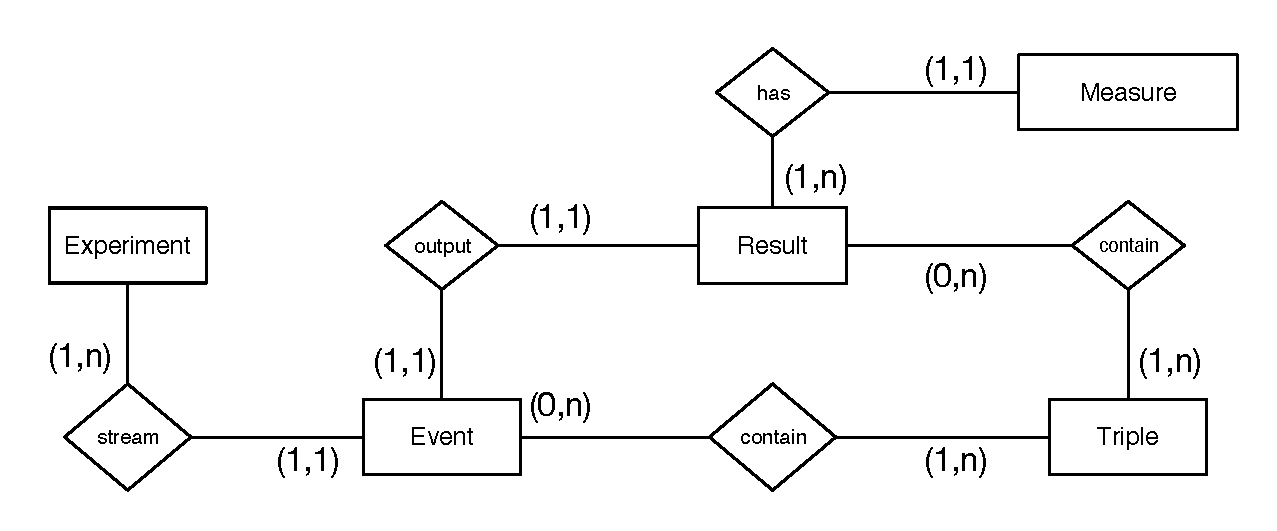
\includegraphics[width=\linewidth]{images/er-db}
	\caption{ER-Diagram For Experiment Output} 
  	\label{fig:er}
\end{figure}\\
\noindent\textsc{Experiment}(\underline{ID}, Timestamp Start, Timestamp End, Engine, Ontology, Query, Dataset, Description)\\
\textsc{Event}(\underline{ID, Experiment ID}, Timestamp)\\
\textsc{Result}(\underline{Result ID, Experiment ID}, Event ID)\\
\textsc{Measure}(\underline{ID}, Value)\\
\textsc{Measurement Set}(\underline{Measure ID, Result ID, Experiment ID})\\
\textsc{Triple}(\underline{S,P,O})\\
\textsc{Output Triple}(\underline{Result ID, Experiment ID, S, P, O})\\
\textsc{Input Triple}(\underline{Event ID, Experiment ID, S, P, O})\\

The \textsc{Experiment} entity contains all the metadata of the tuple $<\mathcal{E},\mathcal{D},\mathcal{T},\mathcal{Q},>$, which semantic is explained above. "Timestamp Start" and "Timestamp End" are relevant metrics for further analysis and system control. 
The \textsc{Event} is unique inside an \textsc{Experiment}, it is possible to send two events with the same timestamp and identical tripleset. The \textsc{Result}  is associated with one and only one \textsc{Event}. It contains the results to the engine queries w.r.t the active window and the set of the measure gathered during the execution. The \textsc{Measurement Set} table represent the relation between the \textsc{Result} and a number of measure that may variate  to fulfil requirement [R.7] (extendible measurement set). We include the concept of the \textsc{Triple} in order to model the content of \textsc{Event and Result}. \textsc{Input Triple} and \textsc{Output Triple} are the tables which represent the relation between \textsc{Triple} and respectively \textsc{Event} and \textsc{Result}
%a file, which contains a tuple with the sensor data and metadata for each event passed during the experiment execution; a set of TriG files that represents the window materialisation at each cycle, even in case of incremental reasoning. (It is also possible to save the non-materialised window, in order to verify the Completeness and Soundness of the reasoning procedure for the baselines).
%In practice the Test Stand outputs results in time series format and  the Analyser toolset has to handle this kind of information. 

\noindent The \textsc{Test Stand} orchestrates the communication between the upstanding models, forcing the \textsc{Streamer} to push events to the RSP Engine and the \textsc{Result Collector} to listen the output and collect the results.  To explain its workflow we split the process at the points when the modules exchange events. Indeed, each message represents a different logic step in the experiment execution cycle and we have distinguished six different ones.

In step (1) the \textsc{Test Stand} take the experiment and start the execution.  The \textsc{Test Stand} executes the experiment $<\mathcal{E},\mathcal{D},\mathcal{T},\mathcal{Q},>$ stressing $\mathcal{E}$ for a certain period of time looping through the steps from (2) to (5) illustrated in Figure \ref{fig:architecture}.                                                                                                                                                                                                                                                                                                                                                                                                                                                                                                                                                                                                                                                                                                                                                                                                                                                                                                                                                                                                                                                                                                                                                                                                                                                                                                                                                                                                                                                                                                                                                                                                                                                                                                                                                                                                                                                                                                                                                                                                                                                                                                                                                                                                                                                                                                                                                                                                                                                                                                                                                                                                                                                                                                                                                                                                                                                                                                                                                                                                                                                                                                                                                                                                                                                                                                                                                                                                                                                                                                                                                                                                                                                                                                                                                                                                                                                                                                                                                                                                                                                                                                                                                                                                                                                                                                                                                                                                      

In step (2), the \textsc{Streamer} pushes to $\mathcal{E}$ an event \textsc{CTEvent}. This event is a portion of an RDF Stream picked from the data $\mathcal{D}$ and it consists of a set of RDF triples with the same timestamp. In order to satisfy [R.12], it sends triple in N-Triple\footnote{\url{http://www.w3.org/2001/sw/RDFCore/ntriples/}}, which is the easiest RDF serialisation to parse.  

In step (3) $\mathcal{E}$ pushes to the \textsc{Result Collector} an event \textsc{OutCTEvent}. It contains the current answer to the query $\mathcal{Q}$ registered in $\mathcal{E}$ given the ontology $\mathcal{T}$. The \textsc{Test Stand} expects $\mathcal{E}$ to output result in N-Triple format. 

Notably, to place any RSP engine on the \textsc{Test Stand} (requirement [R.3]) \name provides a simple software wrapper that, when it receives a \textsc{CTEvent}, adapts it to the RSP engine specific format, pushes it in the RSP engine, and listens to the RSP engine output so to transform such an output in a \textsc{OutCTEvent}.

To measure performances (requirement [R.6]) the \textsc{Test Stand} performs several actions both before step (2) and after step (3) to collect data from the sensors. In step (4), those observations are added to the outputs of $\mathcal{E}$ as annotations and are pushed to the \textsc{Result Collector}.  We name \textsc{TSResult} the event that contains the sensor data plus the query results produced by the engine.  The \textsc{Test Stand} works in a single thread mode, blocking the execution of its components when it performs the measurements in (2) and (3) [R.4].  

Previous works about Stream reasoning \cite{} shows that the minimal performance measure set includes \textbf{Latency} -- defined as the delay between the injection of an event in the RSP engine and its response to it --, \textbf{Memory Load} -- defined as the difference between total system memory and the free one --, and \textbf{Completeness \& Soundness} of query-answering results. To measure latency, it starts a timer before (2) and stops it after (3). To measure memory load, it asks for the free memory of the system after step (3).

In step (5) the \textsc{Result Collector} saves \textsc{TSResult} for post process analysis [R.9], executed trough the \textsc{Analyzer}. It does so saving the content of any TSResult  [R.8].

\section{Baselines}
\label{sec:baselines}

\noindent In Chapter \ref{chap:problem-settings} we state that a Systematic Comparative Research Approach needs initial terms of comparison to lead the investigation. \name contains a set simple and easy-to-use RSP Engines called "baselines", developed to fulfil this lack . 
We exploit them to define some qualitative methods of investigation and to prove the usability of the Test Stand. 

In section \ref{sec:requirements} we identifies four characteristics that classify a case-study as a baseline inside a research field and here we report how \name Baselines are \textit{Elementary}, \textit{Relevant}, \textit{Simple} and \textit{Eligible}.

Early works on SR \cite{DBLP:conf/fis/ValleCBBC08,Walavalkar08streamingknowledge} describe the most simple approach to create a stream reasoning system: pipelining a DSMS with a reasoner. The DSMS is responsible to handle the data stream, moving from infinite sequences to finite (and processable) sets of events. The reasoner instead applies SPARQL queries on this set of events, exploiting its reasoning capabilities over a context that can be considered as static, but remains continuous.  As explained in Section \ref{sec:sfp}, we focus on this three the Stream Reasoning main building blocks: \begin{enumerate}
\item[1.] RDF streams;
\item[2.] An extensions of SPARQL to manage continuos data
\item[3.] reasoning algorithms
\end{enumerate}

\begin{figure}[tbh]
  \centering
	\includegraphics[width=\linewidth]{images/baselines-final}
	\caption{A: the architecture of the Naive baselines. B: the one of  the Incremental ones.} 
  	\label{fig:baselines}
\end{figure}
These there elements are summarised into RSP Engines, systems that can apply reasoning techniques upon rapidly changing information (Section \ref{sec:rspengine}). The approach above allow to develop an RSP Engine focusing only on link two existing technologies and develop the communication between them. But, how this design model fulfil the requirements poses in Section \ref{sec:requirements}?

Baselines \textit{Elementarity} is easy to be granted. The architecture above demands to choose a  DSMS which is a reliable solution in the CEP context  and the a general purpose rule engine which can be consider in the same way. We can consider this goal as reached when the couple elements are simple and valid terms of comparison w.r.t the state of the art.  Baselines \textit{Relevance} means to cover all the most important theoretical variants that the "pipeline approach" conveys. In terms of reasoning we can choose between to possible approaches and with reference to the data stream processing we have again two choice. Four baseline implementations cover these two main design decisions about the RDF Stream Model and the Reasoning procedures. 

The RDF Stream model describes how the input RDF Stream is processed, different systems accept data in different models, which depends on how RDF Stream is considered in terms of events contemporaneity. The two most relevant ones are:

\begin{itemize}	
\item Triple-based model, where the events pushed in the DSMS are timestamped triples. The timestamps are non decreasing, different triples could have the same timestamp to denote that they are contemporary.
\item RDF Graphs-based: the event pushed in the DSMS are timestamped RDF graph. The timestamps are increasing and the graph is used as a form of punctuation \cite{Tatbul2003b} to separate consequent portions of the RDF stream.
\end{itemize}

The Reasoning Architecture, the techniques to make inference, depends on the way data flow from the DSMS to the reasoner. Two reasoning solutions exist for the two triples data flow:

\begin{itemize}
\item Naive solution: (Figure \ref{fig:baselines}-A) the DSMS produces an RDF Snapshot of the current windows. Tt sends the entire content of the window to the reasoner, which materialises all the implied triples at each cycle. This is the approach implemented in the C-SPARQL Engine \cite{DBLP:journals/sigmod/BarbieriBCVG10} and in Sparkwave \cite{DBLP:conf/debs/KomazecCF12}.
\item Incremental solution (Figure \ref{fig:baselines}-B) the DSMS outputs the IRStream, the differences between the current window and the previous one. The $\Delta^{+}$ snapshot contains the triples that have just entered in the window, while the $\Delta^{-}$ snapshot contains the triples that have just exited from the window. The reasoner, using $\Delta^{+}$ and $\Delta^{-}$, incrementally maintains the materialisation over time. This approach is taken as term of comparison in \cite{DellAglio2014} and it is inspired from \cite{DBLP:conf/cikm/RenP11}.
\end{itemize}

Baseline \textsc{Eligibility} requires to check out all the performance measurements involved by the RSP Engine in use. We already stated that the choice of the DSMS and the reasoned may affect baseline \textsc{Elementarily}, but they also influence the performance of the engine. As reported in Section \ref{sec:teststand}, we take as initial measure set: Latency, Memory and of the query results Completeness and Soundness. The baselines must be at least comparable with commercial solutions in terms of degree of magnitude, in order to be Eligible for Latency and Memory. More consideration on this metrics are presented in Chapter of \ref{chap:evaluation}, which deeply answers the question with experimental results. On correctness of RDF stream processing \cite{DBLP:conf/semweb/DellAglioCBCV13} previous works explain the importance of external control on time to assure that the RSP Engine always outputs the correct answers (even when overloaded). The proposed baselines should take advantage of the ability of some DSMS to be temporally controlled by an external agent by sending time-keeping events to synchronise the internal time flow. %One time-keeping event is sent before injecting the triples in a \textsc{TCEvent} and another one after all triples in \textsc{TCEvent}  were sent. In this way all the triples in the TCEvent are consider contemporary by the 

Finally, baselines \textsc{Simplicity} comes from those parameters that directly influence the RSP Engine: the query $\mathcal{Q},$ and the entailment regime. $\mathcal{Q}$ should be eligible in terms of reasoning which means having an high materialisation effort of the implicit information entailed by the content of the window, given the ontology chosen by the user. The entailment regime should be a fragment of a language, maybe RDF-S,  which reduce complexity but preserves the normative semantics and the core functionalities. Moreover, what we state above about externally time control clarify the system workflow, so it is demanded to sustain baselines \textsc{Simplicity} too.

\section{Analyser}\label{sec:analyser}

The \textsc{Analyser} consists, from an engineering point of view, in one or more automated procedures which process the experiment results transforming raw data into an human-readable form. Actually, not all the analysing procedures can be completely automated and data analysis can not be always generalised. 

From a research point of view instead, the \textsc{Analyser} consists in a set of methods for data processing and analysing, which allow to refute or confirm hypothesis and improve existing models trough empirical findings.

In this Section we focus on the definition of the methods that compose the analysis, while in Section \ref{sec:analyser-impl} we detail much more which tools sustain the investigation at different levels, allowing data visualisation and deeper statistical investigations. \\

\begin{figure}[tbh]
  \centering
	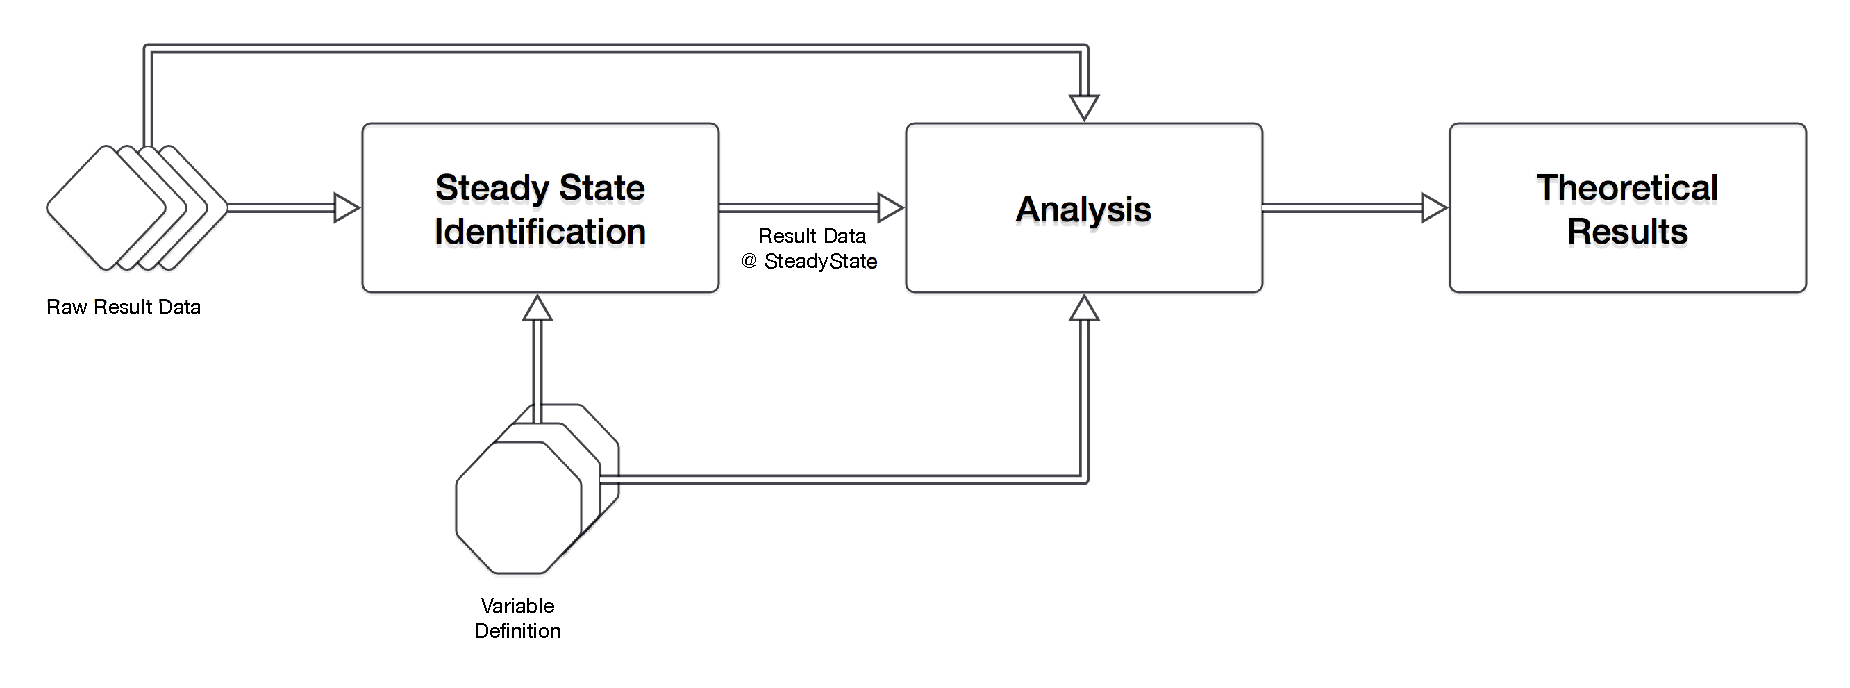
\includegraphics[width=\linewidth]{images/analyser-block-schema}
	\caption{From raw data processing to Theoretical results} 
  	\label{fig:analyser-block-schema}
\end{figure}

Figure \ref{fig:analyser-block-schema} shows the different phases of the data processing. The methods that compose the \textsc{Analyser} can be divided into three main steps, each one with different supporting tools and different goals.

\textsc{Analyser} takes as input the raw data produced by the \textsc{Test Stand} executing experiment, and the variable on which the analysis will be based on. In Section \ref{sec:teststand} we have described the \textsc{Test Stand} workflow. It outputs in times series form the data it gathers during the execution of an experiment. Which data the \textsc{Test Stand} gathers, the variable of the analysis, depend on the sensors it contains. To this extent the \textsc{Analyser} must parametric from the variable analysis. 

The First step in Figure \ref{fig:analyser-block-schema} is the \textit{Steady State Identification}, which can be seen as a pre-processing of the raw data.

\begin{figure}[tbh]
  \centering
	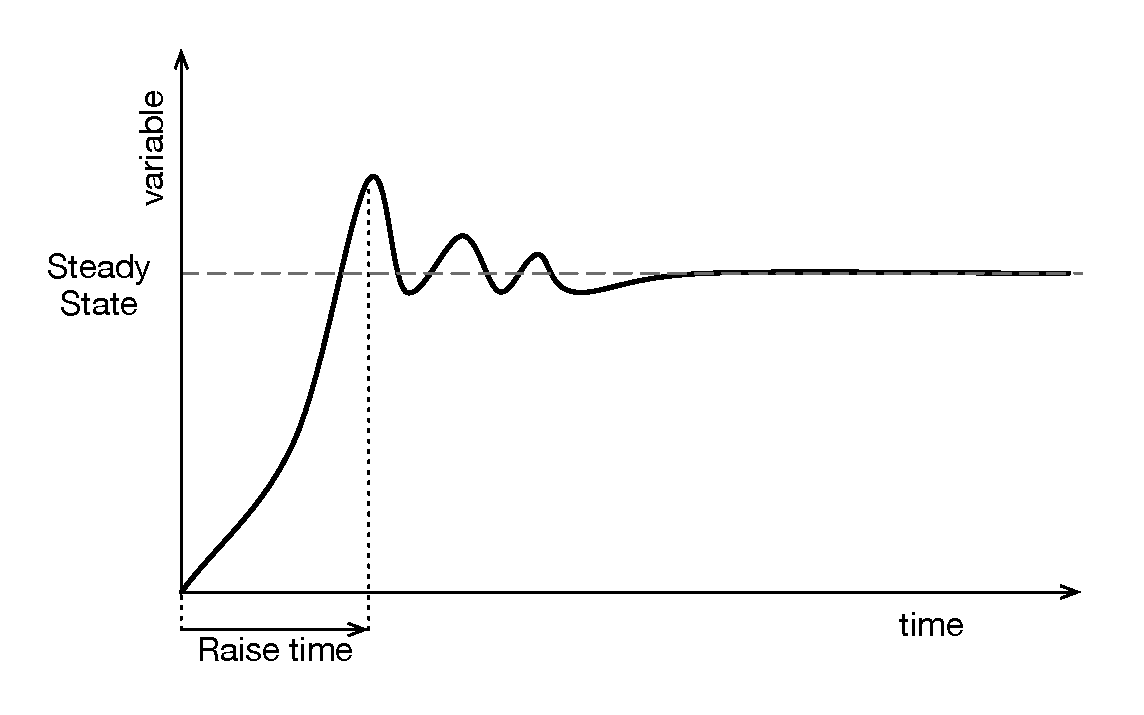
\includegraphics[width=0.5\linewidth]{images/steady-state}
	\caption{Time Series temporal domain} 	
  	\label{fig:steady-state}
\end{figure}

The Steady State is the moment when a dynamic system reaches the equilibrium for a certain variable. The identification of this condition is a common passage in almost any research on dynamic system and visual analysis can be exploited as the simplest tool to complete the task. Figure \ref{fig:steady-state} shows the typical behaviour in the time domain for a certain variable and also evidences the point when the the serie reaches the Steady State condition. Dynamic systems usually have an initial warm-up phase which negatively influences results and inhibit generalisation and comparisons. To properly contrasts results between $n$ different RSP Engines data must be standardized. In the \textit{Steady State Identification} step data are processed according to the variable definition, identifying which variable has reached a steady state condition. The Steady state identification process allow to understand the degree of reliability of the data, how we can assume a certain observation is confirmed and generalizable. 


Once the Steady State is identified is possible to proceed with data processing, which is summarised in Figure \ref{fig:analyser-block-schema} by the Analysis step. The analysis process all the data, but we distinguish the analysis w.r.t. the results form Steady State Identification step, because the analysis of the warm-up phase is a crucial part of the system comprehension and thus of the Hypothesis confirmation, as we will see in Chapter \ref{chap:evaluation}.


The last step in the high level Analyser process is consist in the formalisation of theoretical results. The aim of this step is obviously confirm or refute hypothesis formulated at experiment design level. However, \name has the aim of sustaining the empirical research which allow a new kind of observation that may improve existing theoretical model, changing the meaning of old hypothesis.

\subsection{Analysis Step}

The Analysis step we introduced above represents the concrete processing of the experiment result data. In this Section we detail this step. We decompose the analysis in four levels of different analysis details. We  introduce different analysis methods that each level involves. Figure \ref{fig:analysis-method} is a graphical representation of the Analysis stack, where the detail level grows from the top to the bottom. Further levels may be introduced at any point in the stack, since this design comes from the formalisation of our research work onver the Baselines presented in Chapter \ref{chap:evaluation}.

\pagebreak

Before presenting the stack level one by one, we introduce two concept about the experiment analysis:
\begin{itemize}
\item \textit{Intra Experiment Comparison} -  it means comparing results of different solutions (RSP Engine) within a single experiment, fixing only $\mathcal{D}, \mathcal{T} $ and $\mathcal{Q}$ or comparing different variables of the same solution  in a certain experiment.
\item \textit{Inter Experiment Comparison} -  it means comparing the same solution (RSP Engine) in different experiments or comparing how different solutions changes their behaviour in different experiments
\end{itemize}

\begin{figure}[tbh]
  \centering
	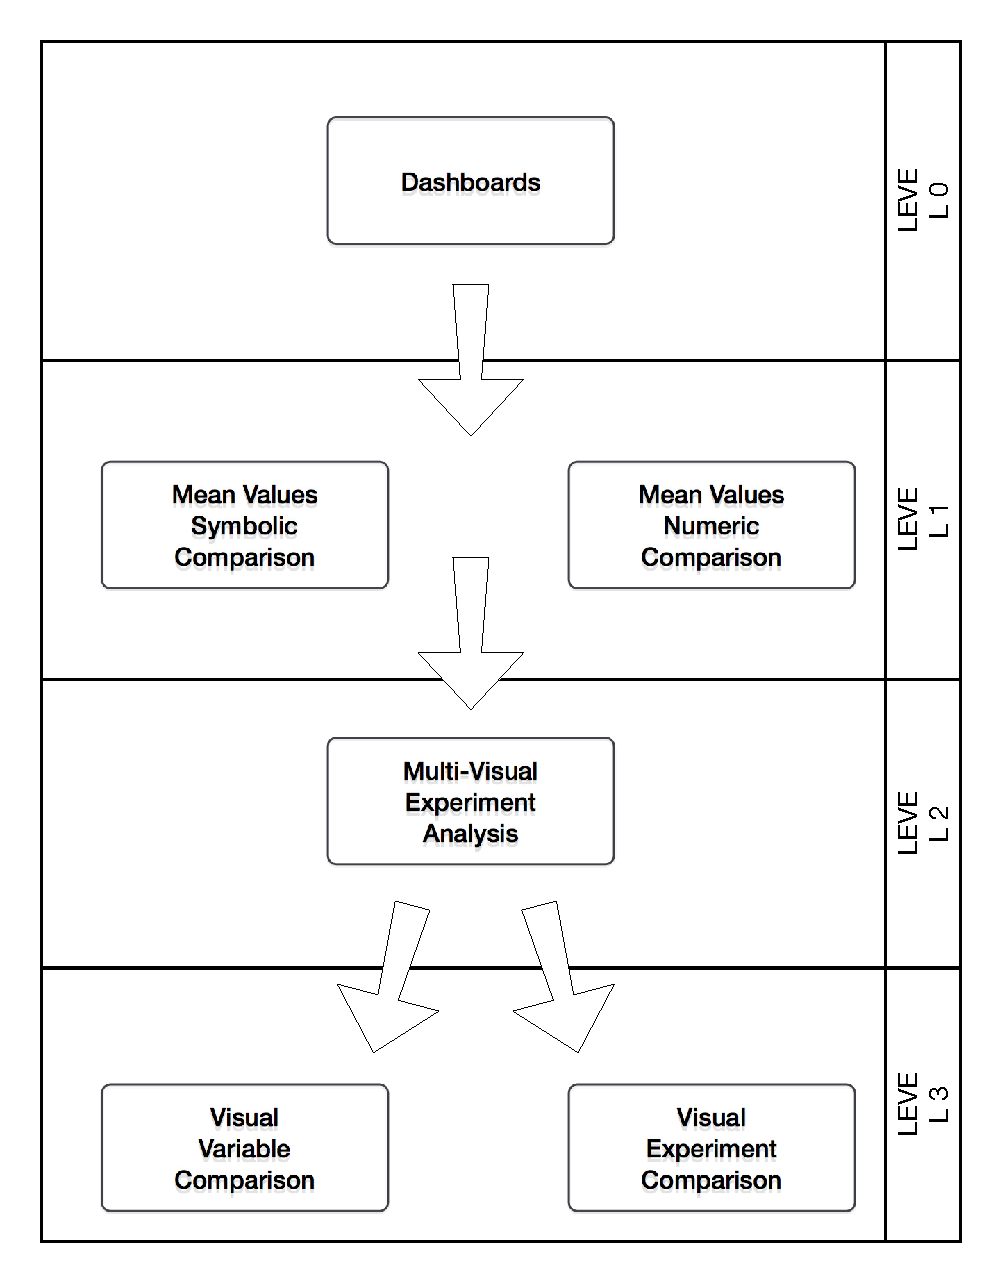
\includegraphics[width=\linewidth]{images/analysis-method}
	\caption{Analysis method stack. The level of analysis grows from the top to the bottom} 
  	\label{fig:analysis-method}
\end{figure}


\textsc{Level 0 - Dashboards}\\

Dashboards are the highest level of analysis offered by \namens. The Mean data value are presented in a n-dimension radar plot, which involves all the variables selected during the experiment design phase. Visual comparison of the data trough dashboards is natural when few variable are involved. It is easy to compare many solution and identify which one is the best, if any. Dashboard allow both inter-experiment comparison and intra-experiment comparison. 

The idea of a single visualisation method which allow to answer to any hypothesis is desirable, but not probable.  Unfortunately, the reliability of the methods depends on the system complexity and no only on the complexity of the method itself. Usually this level of analysis can not represent the entire system complexity. Moreover, if the Steady State condition is not reached by all the variable involved, the generalisation of any insight may be difficult. Further levels of analysis are required, at least for a better comprehension of those unpredictable results that refute even naive hypothesis, formulated on well known theoretical truths.

\textsc{Level 1 - Mean Value Comparison}\\

This Analysis level focuses on a single variable a time, exploiting both \textit{Intra-Experiment} and \textit{Inter-Experiment} comparison. Usually hypothesis verification requires the definition of multiple experiment, which variates for on or more parameters. This kind of analysis split  the dashboard representation, presenting one variable at time, comparing the results of different solutions.

Usually this comparison involves multiple experiment, presented in a easy-to-ready form, which evidence the differences between experiments.

\name makes possible two approach of this kind of analysis:
\begin{itemize}
\item \textit{Numeric} -  The comparison results are present in percentage form, quantifying how much a solution is better than another one, fixing some elements in the experiment.  With Numeric Mean variable comparison is possible to see how much, for a certain variable, the improvement of a given solution changes between experiment w.r.t. another one.

\item \textit{Symbolic} - it is a simplification of the Numeric Solution. Sometimes we only need no understand which solution is better, without focusing on numerical value. Symbolic solution required the definition of a tolerance threshold, for example 5\%, to distinguish when a solution is better, worst or equal to another one.

\end{itemize}
\textsc{Level 2 - Multi-Visual Experiment}\\


\textsc{Level 3 - Visual Comparison}\\
\begin{itemize}
\item \textit{Variable Comparison}
\item \textit{Experiment Comparison}
\end{itemize}






 \clearemptydoublepage
%\section{Heaven}\label{sec:impl-intro}

The architecture of the \textsc{Test Stand} consists in three stand alone modules that establish a mono-directional communication flow: \textsc{Streamer}, \textsc{RSP Engine} and \textsc{Result Collector}. Some of the requirements reported in Section \ref{sec:requirements} directly affect the implementation experience of \name and Chapter \ref{chap:heaven} describes how fulfil them. First of all the requirements [R.10], i.e. the need of an \textit{Extendible Design}, and [R.11], which states the necessity of an \textit{Event-base architecture} to properly face any RSPEngine, are immediately relevant. 

To be \textit{Extendible} the \textsc{Test Stand} requires two main abstractions: the \textit{Event} and the \textit{EventProcessor}.

\textit{Event} concept is required to build a hierarchical communication. Indeed, the \textsc{Test Stand} may handle three events flows: one internal to the RSP Engine module, one for the communication between modules and one to communicate with the user. Next section about data clarifies the communication structured. 

The \textit{Event Processor} guarantees the system to be modular, it standardizes the interaction simplifying the behaviour of each component in the system. 

Thus, a module is an \textit{Event Processor} which can be positioned everywhere in the the \textsc{Test Stand} pipeline. % As a matter of facts, specific implementations of a module may reduce the generality of this definition and also the flexibility of the module itself.	

\begin{figure}[tbh]
  \centering
	\includegraphics[width=\linewidth]{images/fsm-schema}
	\caption[\textit{EventProcessor} States Diagram]{The finite state machine diagram of the \textit{EventProcessor} interface module}
  	\label{fig:module-fsm}
\end{figure}

The requirement [R.4] states the \textsc{Test Stand} \textit{must not be running when the RSP Engine is under execution} (see Section \ref{sec:requirements}) conditioning \name workflow. To cover [R.4] we designed the status of each module  as a Finite State Machine (FSM), which can work only in those states that allow processing (READY). The schema in Figure \ref{fig:module-fsm} represents the FSM for each module of \name, even the Baselines, and also for the \textsc{Test Stand} external structure. 


The \textit{Startable} Interface standardize two methods, \textit{init()} and \textit{close() }which allow to control the behaviour of the Module at the start and the end of the execution. The interface allows to move from the CLOSED state to the READY trough the \textit{init()} method, it moves from the READY to the CLOSED trough the \textit{close()} method. 

We state that each module is an \textit{EventProcessor}, which also implements the \textit{Startable} Interface. THe \textit{process (Event e)} brings the module into the RUNNING state until the processing ends, and then back to the READY one. One and only one module can be in the RUNNING state in a certain moment during the execution. This behaviour is exploited by the \textsc{Test Stand} external structure to control execution fulfilling [R.4] by stopping its process while the RSP Engine is running (see Section \ref{sec:teststand}). ERROR State, which can be reached from any point of the execution, prevents the propagation of errors over result data: when a module fails the execution is stopped without saving the erroneous data (last event) and reporting the error to the user.

\section{Events and Data}\label{sec:data-impl}

Chapter \ref{chap:problem-settings} poses the requirements of an Event-based architecture [R.11] for the \textsc{Test Stand}. Moreover, Chapter \ref{chap:heaven} describes \name workflow and how it exchanges events during the execution. The \textsc{Test Stand} modules interact trough events, see \ref{fig:uml_events},  which contains data at different points of the experiment process. \name handles three kind of events:

\begin{figure}[tbh]
  \centering
	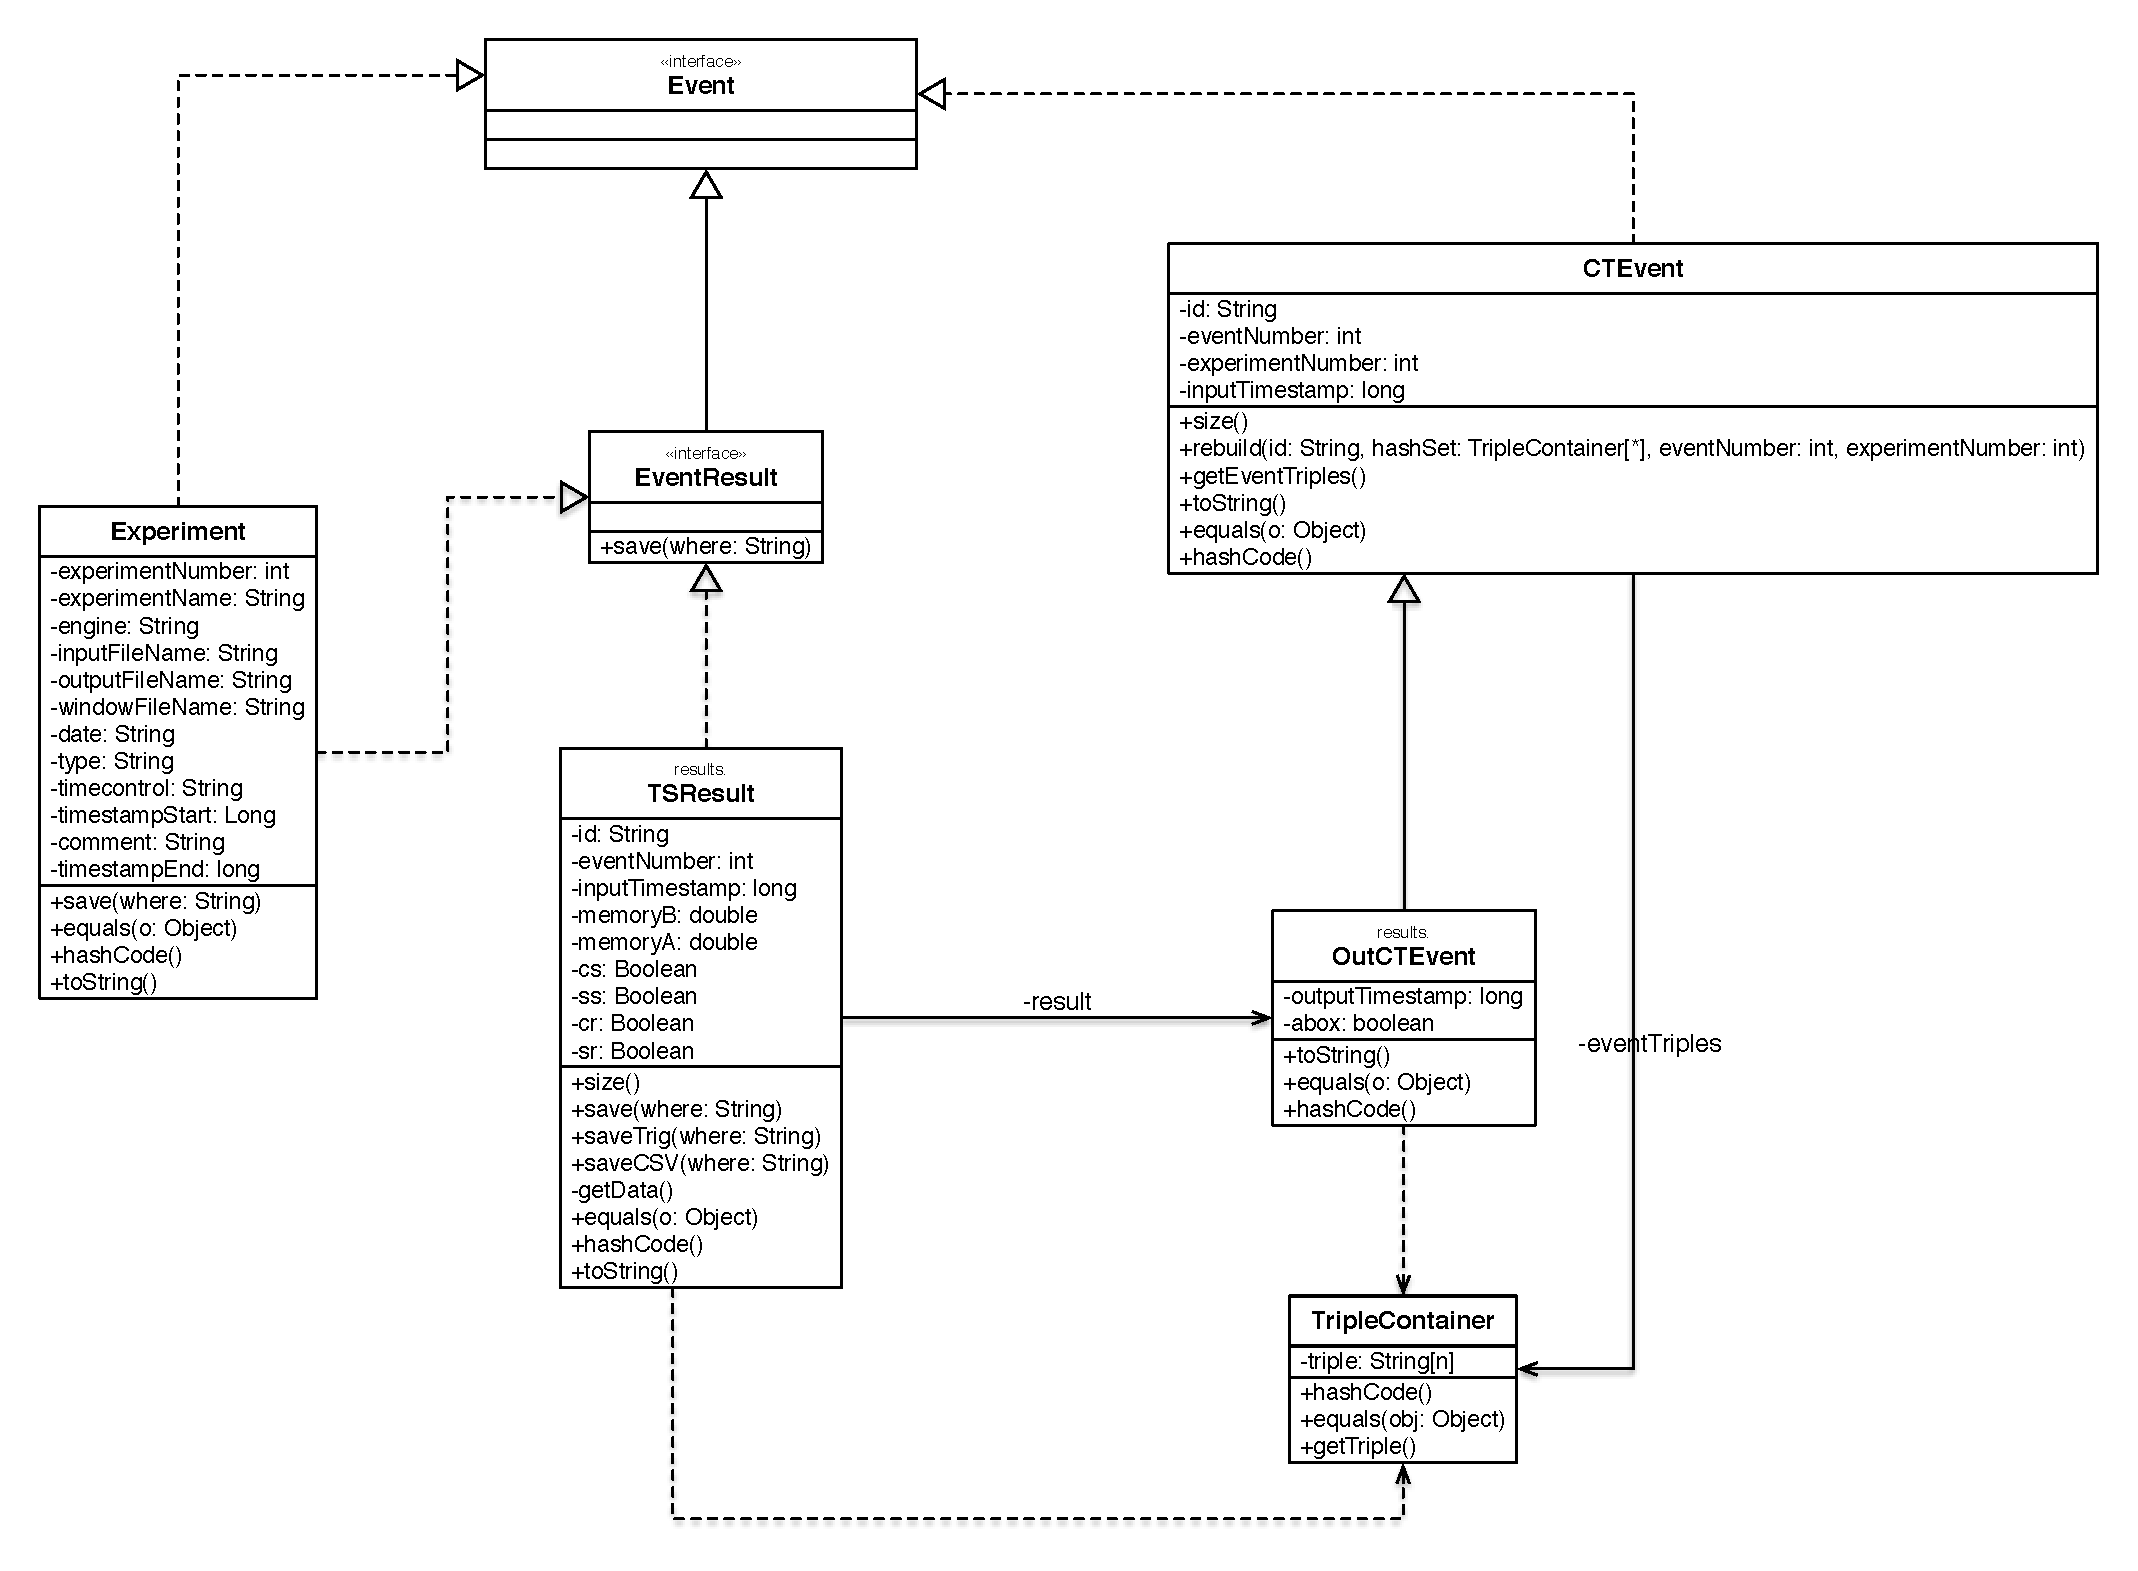
\includegraphics[width=\linewidth]{images/uml_events}
	\caption[\name Execution Events - UML Schema]{The figure shows the event that \name \textsc{Test Stand} and its modules 	exchanges during the execution of an experiment. All of them implement the \textit{Event} interfaces that start the class 	hierarchy.} 
	\label{fig:uml_events}
\end{figure}

\begin{itemize}
\item \textit{Experiment} - it represents the tuple $<\mathcal{E}, \mathcal{D},\mathcal{T},\mathcal{Q}>$, indicating which RSP Engine will be tested and with which queries, data and ontology will be used. It indicates if the current implementation of the engine exploit external timing. Finally the $type$ parameter indicates which kind of testing will be applied (SOAK o Stress for example) and it contains also the execution start time or end time.
\item \textit{CTEvent} - it contains a set of contemporary triples, wrapped in the \textit{TripleContainer}, which allows us to redefined hashcode and equals as a relation of the subject, object and predicate of the RDF triple. The id identifies the event within the experiment.
\item \textit{OutCTEvent} - it represents the event produced by the RSPEngine after processing the active window. Figure \ref{fig:uml_events} show the inheritance relation between \textit{CTEvent}:  \textit{OutCTEvent} extends the \textit{CTEvent} adding the outputTimestamp field.
\item \textit{TSResult} - it wraps the \textit{OutCTEvent} adding the information about the minimal sensor data: memory, sampled ante e post processing, and latency. Two boolean fields allow complete and soundness result, if it is evaluated at runtime (see Section \ref{sec:requirements})
\end{itemize}

\name requires an initialization phase to prepare and input the \textit{Experiment} into the \textsc{Test Stand}. The current implementation exploits a property file with the Experiment parameters: ID and the tuple $<\mathcal{E}, \mathcal{D},\mathcal{T},\mathcal{Q}>$. 

The \textit{CTEvent} and the \textit{OutCTEvent} contain RDF triples in NT-Triple\footnote{http://www.w3.org/2001/sw/RDFCore/ntriples/}, which is the easiest RDF serialisation to parse. This serialisation was chosen to fulfil requirement [R.12], which demands an \textit{Easy-to-Parse RDF Serialisation for the events presented to the RSP Engine in exam}. Figure \ref{fig:uml_events} shows also that the RDF Triples are stored in the events into the \textit{TripleContainer} wrapper: we redefine the triple hashcode and equals method guaranteeing their uniqueness of within an \textit{CTEvent} or \textit{OutCTEvent}.

\section{Modules}\label{sec:modules-impl}

In this section we present the three modules which compose \name: the \textsc{Streamer},  the \textsc{ResultCollector} and the  \textsc{Test Stand Supporting Structure}. They all extend the \textit{EventProcessor} and the \textit{Startable} interfaces.

In Section \ref{sec:impl-intro} we define a module a an \textit{Event Processor} which can be positioned everywhere in the the \textsc{Test Stand} pipeline. We state that a module must implements the \textit{Startable} interface, which completes the FSM schema in Figure \ref{fig:module-fsm} with the \textit{init()} and \textit{close()} methods.
Thus, each modules in this section offers three standard methods to interact with them: \textit{process(Event e)} from \textit{EventProcessor} and \textit{init()} and \textit{close()} from the \textit{Startable} Interface.

\subsection{Streamer}	\label{sec:streamer-impl}
\begin{figure}[tbh]
  \centering
	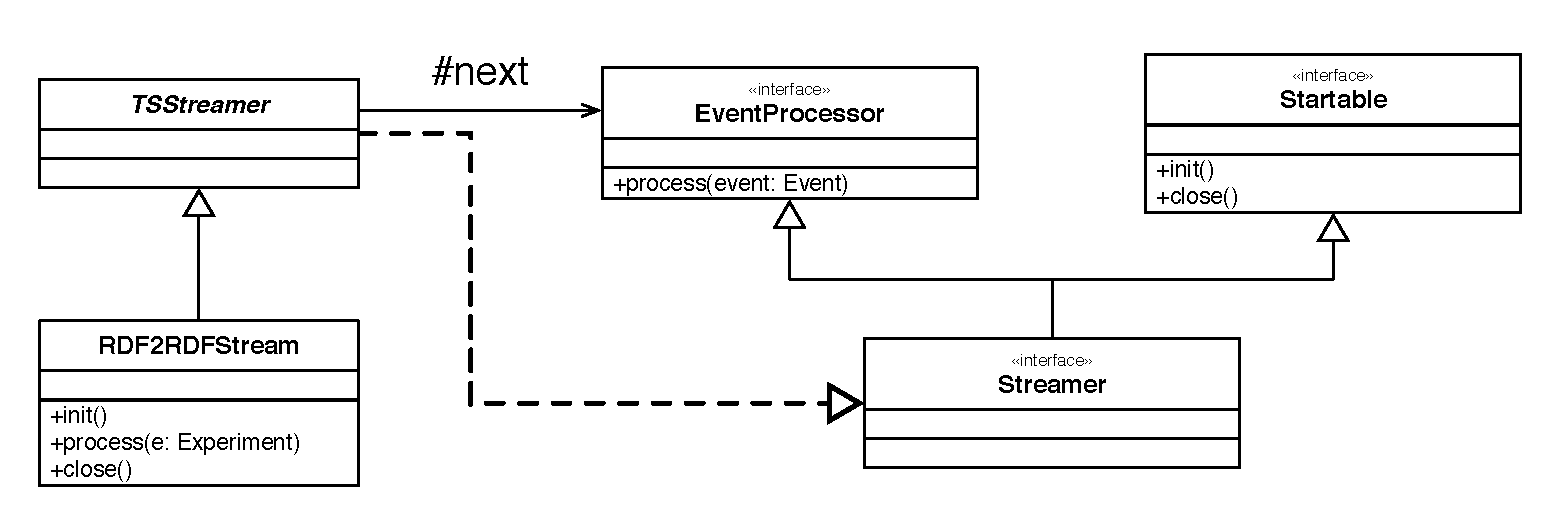
\includegraphics[width=\linewidth]{images/uml_tstreamer}
	\caption[\textit{RDF2RDFStream \textsc{Streamer} Implementation} - UML Schema]{Current implementation of the \textsc{Streamer} module. \textit{RDF2RDFStream} extends the \textit{TSStreamer} abstract class, which defines the module as an \textit{EventProcessor} of \textit{Experiment}s} 
  	\label{fig:uml_tstreamer}
\end{figure}

\noindent Figure \ref{fig:uml_tstreamer} shows the current implementation of the \textit{Streamer} interface, which starts the \textsc{Test Stand} pipeline. Actually, the \textit{Streamer} is implemented as the \textit{TSStreamer} abstract class, which specialises the event processing to the class \textit{Experiment}. 

The \textit{Experiment}s eveant that the \textit{TSStreamer} receives are instantiated externally. The module can start the processing only once it is initialised, then it communicates with one referenced \textit{EventProcessor}, called \textit{next}, which is represented in Figure \ref{fig:uml_tstreamer} by the labelled arrow. The \textit{next} process \textit{CTEvent}s. The nature of the communication between the\textit{TSStreamer} and the following \textit{EventProcessor} depends on the user needs. Notice that also the \textit{next} must be initialised before starting the communication, otherwise the ERROR state will be reached when the event is received by the \textit{next}, because the processing is not allowed.

Figure \ref{fig:uml_tstreamer} contains also the \textit{RDF2RDFStream} implementation, whose internal structure can be seen in Figure \ref{fig:uml_flowrateprofiler}. The \textit{RDF2RDFStream} was developed to conduct experiments as they are presented in Chapter \ref{chap:evaluation}.  It is worth to note that we use LUBM Benchmarks to generate the data for the experiments. LUBM generated data are static, thus the \textit{RDF2RDFStream} builds an RDFStream attaching a timestamp to the static data produced by LUBM. %The file is generated using  LUBM(1000,0), which means 1000 different universities with the random generation seed 0. 

\begin{figure}[tbh]
  \centering
	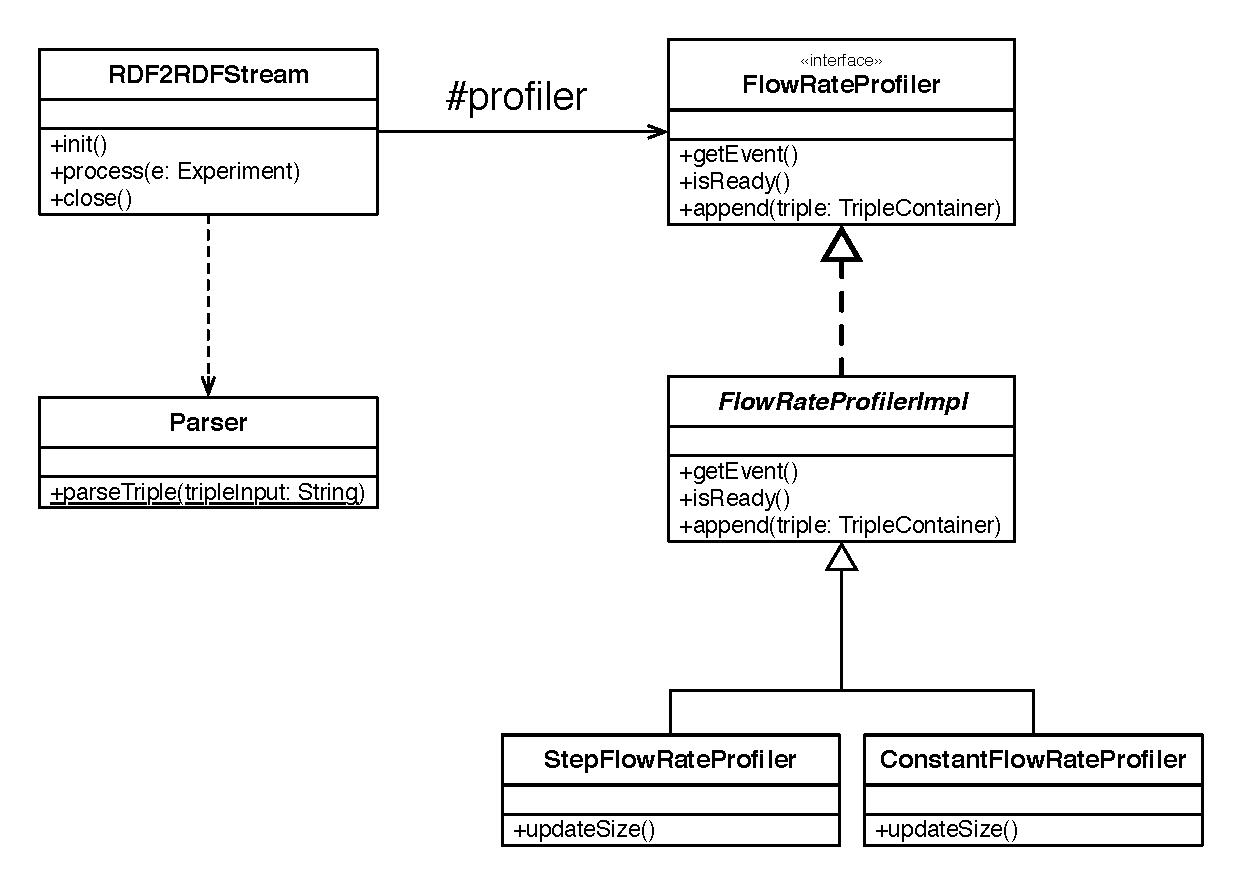
\includegraphics[width=0.75\linewidth]{images/uml_flowrateprofiler}
	\caption[Internal Components of \textit{RDF2RDFStream} - UML Schema]{The \textit{RDF2RDFStream} exploits two subcomponents to build an RDF Stream: the \textit{Parser}, which allows to ready in memory RDF Triples, and the \textit{FlowRateProfiler}, which attaches to RDF triple a timestemp and it builds \textit{CTEvent}s according to a function $f=f(x)$. The \textit{FlowRateProfileImpl} provides implementation of the \textit{append(TripleContainer tc}) method and of the two utility methods \textit{isReady()} and \textit{getEvent()}. Specific implementations of the \textit{FlowRateProfiler} control the function $f$ trough the \textit{updateSize()} method.} 
  	\label{fig:uml_flowrateprofiler}
\end{figure}


The \textit{Parser} component, in Figure \ref{fig:uml_flowrateprofiler} can be accessed statically. It reads in memory one by one the triples in the file guaranteeing data independence [R.1] and it does not influence the memory footprint [R.5] by allocating only the memory necessary to parse a triple. 

Figure \ref{fig:uml_flowrateprofiler} also includes the \textit{FlowRateProfiler}. This component determines the number of triples to add to a \textit{CTEvent} and it builds such an event. The In this way, \textit{RDF2RDFStream} can generate different RDF streams to use as $\mathcal{D}$, which differ on the number of contemporary triples in the stream. 

\begin{figure}[tbh]
\centering
\subfigure[Exponential Growing \textsc{CTEvent} Size: $y=2^x$]{
\begin{tikzpicture}
  \begin{axis}[ 
  width=0.4\linewidth,
      height=0.4\textwidth,
    xlabel=$CTEvent$,
    ylabel={$CTEvent Size$},
    xmin=0.00, xmax=40,
	ymin=0, ymax=1048576
  ] 
    \addplot [
    line width=0.75pt]
    coordinates {
    		(0.00, 1.00)
		(1.00, 2.00)
		(2.00, 4.00)
		(3.00, 8.00)
		(4.00, 16.00)
		(5.00, 32.00)
		(6.00, 64.00)
		(7.00, 128.00)
		(8.00, 256.00)
		(9.00, 512.00)
		(10.00, 1024.00)
		(11.00, 2048.00)
		(12.00, 4096.00)
		(13.00, 8192.00)
		(14.00, 16384.00)
		(15.00, 32768.00)
		(16.00, 65536.00)
		(17.00, 131072.00)
		(18.00, 262144.00)
		(19.00, 524288.00)
		(20.00, 1048576.00)
		};	
		
	\end{axis}
\normalsize

\end{tikzpicture}
}
\subfigure[Step Growing Size with K1=100 and K2=1000 after 9 \textsc{CTEvents}]{
\begin{tikzpicture}
  \begin{axis}[ 
  width=0.4\linewidth,
      height=0.4\textwidth,
    xlabel=$CTEvent$,
    ylabel={$CTEvent Size$},
    xmin=0.00, xmax=20,
	ymin=0, ymax=1200
  ] 
    \addplot [
    line width=0.75pt]
    coordinates {
    		(0.00, 100.00)
		(1.00, 100.00)
		(2.00, 100.00)
		(3.00, 100.00)
		(4.00, 100.00)
		(5.00, 100.00)
		(6.00, 100.00)
		(7.00, 100.00)
		(8.00, 100.00)
		(9.00, 100.00)
		(9.00, 1000.00)
		(10.00, 1000.00)
		(11.00, 1000.00)
		(12.00, 1000.00)
		(13.00, 1000.00)
		(14.00, 1000.00)
		(15.00, 1000.00)
		(16.00, 1000.00)
		(17.00, 1000.00)
		(18.00, 1000.00)
		(19.00, 1000.00)
		(20.00, 1000.00)
		};	
		
	\end{axis}
\normalsize

\end{tikzpicture}
}
\caption[Example of FlowRateProfiler Triple Distribution]{The \textsc{FlowRateProfiler} is able to calculate \textsc{CTEvent} size according to a function which relates the number of triple to the number of \textsc{CTEvent}.}
\label{fig:frp-examples}
\end{figure}


The \textit{FlowRateProfilerImpl} implements \textit{FlowRateProfiler} interface. It provides a common implementation for the method \textit{append(TripleContainer tc)}, which adds to the current \textit{CTEvent} an RDF triple,  and of the two utility methods \textit{isReady()} and \textit{getEvent()}. What variates between different implementations of this component, is the \textit{updateSize()} method. The \textit{FlowRateProfiler} creates \textit{CTEvent} according to a function $y=f(x)$, in which $x$ is the number of the \textit{CTEvent} and it results that $y$ is the number of triple this \textit{CTEvent} will contain. The update logic given by $f$ is implemented within the \textit{updateSize()} method. For example if we decide to increase linearly the number of triples inside a \textit{CTEvent} the function $f$ will be: \[y=x, \text{ where } x,y \in N\]
The first event (E0) will contain zero triple, E1 will contain only one triple following E4 will contain four triples and so forth. Another possibility is to increase exponentially the number of triples inside a \textit{CTEvent} : \[y=2^x, \text{ where } x,y \in N\]The first event (E0) will contain one triple, E1 will contain two triple following E3 will contain eight triples and so forth, Figure \ref{fig:frp-examples}.a shows the resulting behaviour plotting the triple number on y-axis and \textit{CTEvent} number on x-axis.



In the current stage of development we include four implementations of the \textit{FlowRateProfiler}, two of them are related to our experiments: 
\begin{itemize}
\item \textit{ConstantFlowRateProfiler} - it maintains the same number of triples for each events over all the experiment: \\
\[y=K, \text{ where } K \in N \]

\item \textit{StepFlowRateProfiler} - it maintains a constant number of triple $K1$ inside a \textit{CTEvents} for $x$ occurrences, then it suddenly changes the number of triple $y$ form $K1$ to $K2$ where $K2 >> K1$. The number of  \textit{CTEvents} $x$ is specified in the set-up phase of the component.  Figure \ref{fig:frp-examples}.b contains the resulting plot of implemented function which follows:

\[
y=
\begin{cases}
K1, &\text{if $x < M$ } $ where $ K1, M \in N\\
K2, &\text{if $x >= M$} $ where $ K2 >> K1, K2 \in N
\end{cases}
\]


\end{itemize}

The remaining two  \textit{FlowRateProfiler} implementations in \name that are not related to our evaluation are:
\begin{itemize}
\item \textit{LinearStepFlowRateProfile} - it streams $x$ \textsc{CTEvents} of dimension $y$, in terms of triples, then linearly increase the number of a quantity $M$: \[y=x*M, \text{ where } x,y,M \in N\]
\item \textit{ConstantRandomFlowRateProfiler} - it changes $y$ and $x$ according with two random integer generators directed by two seeds. The generators provided integer numbers according to a certain probability \[y=randomInt(seed), \text{ where } random(seed),y \in N\]
\end{itemize}


\subsection{Result Collector} 

\noindent The \textsc{ResultCollector} is the data acquisition system that receives and persist the query results and the measurements data gathered by the \textsc{Test Stand} during the execution of an experiment.

\begin{figure}[tbh]
  \centering
	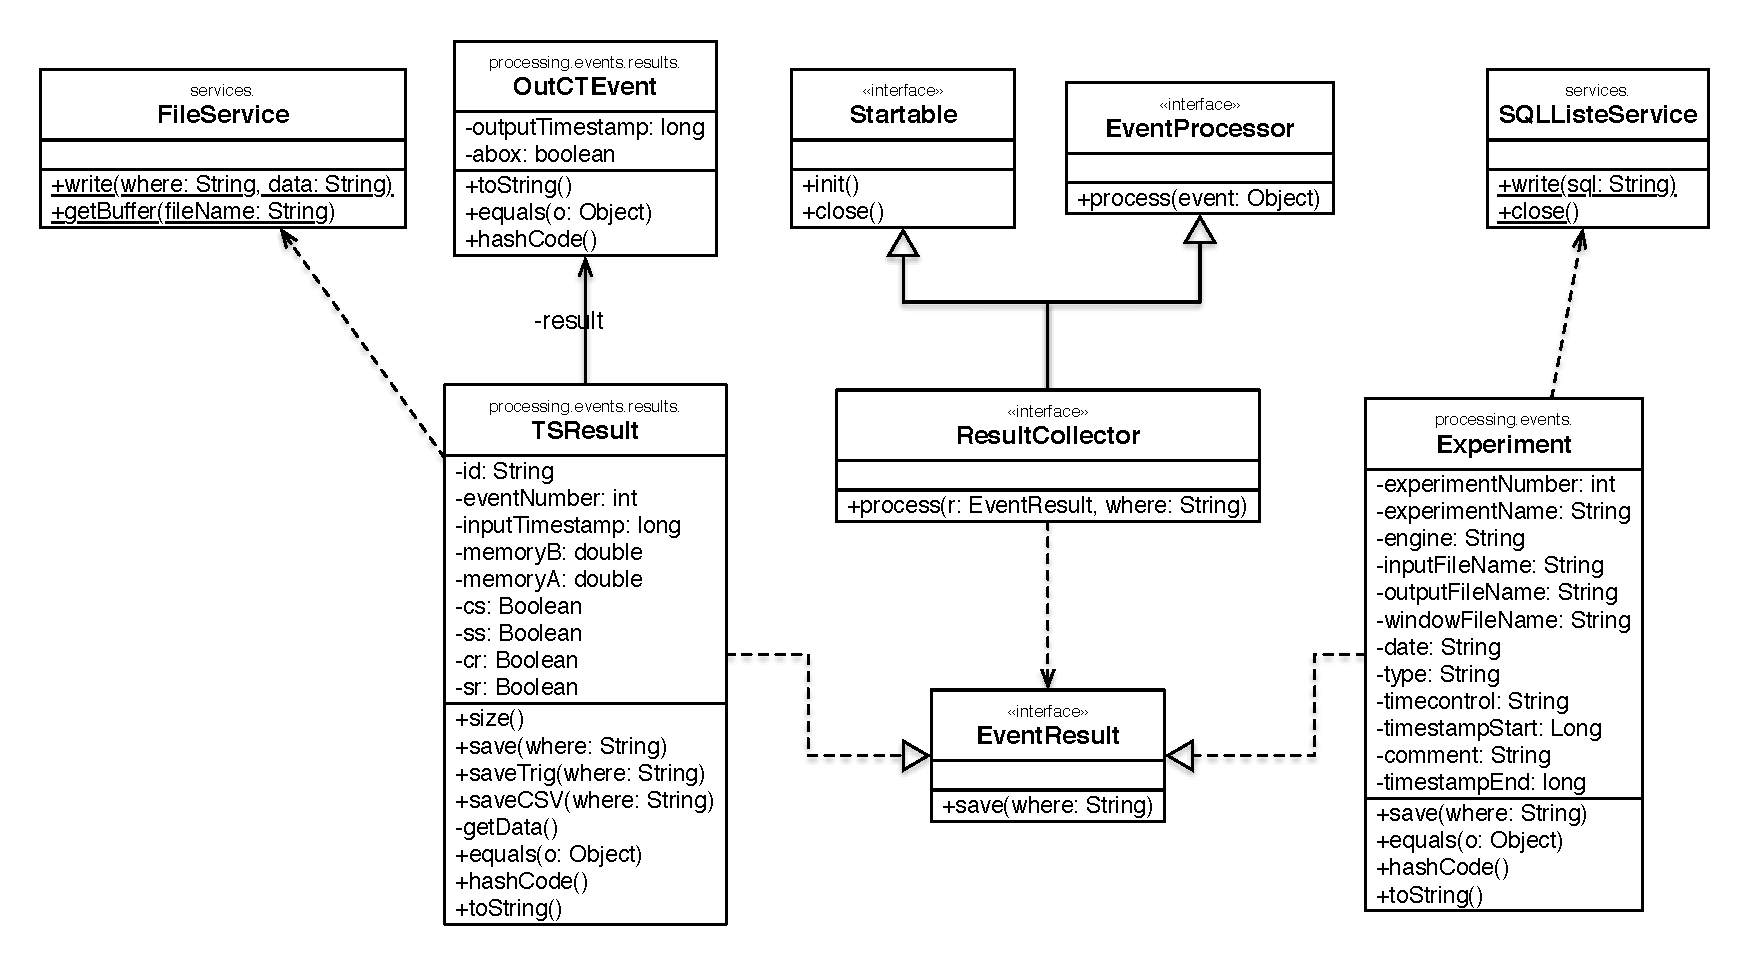
\includegraphics[width=0.5\linewidth]{images/uml_resultcollector}
	\caption[\textsc{ResultCollector} Current Implementation - UML Schema]{The current implementation of the \textsc{ResultCollector} interface is the \textit{TSResultCollector} which processes events that implements the \textit{EventResult Interface}. \textit{ResultEvent} interface hides the saving procedure, delegating the implementation to the event provider trough    the \textit{save()} method. \textit{TSResultCollector} exposes also the method process(Event e, String where), which allows the caller to specify the destination. } 
  	\label{fig:uml_resultcollector}
\end{figure}

The UML Schema in Figure \ref{fig:uml_resultcollector} shows firstly that the \textit{ResultCollector} interface is again an extension of the \textit{EventProcessor} and the \textit{Startable} ones. The current implementation is the \textit{TSResultCollector}, which stays at the end position in the \textsc{Test Stand} pipeline. The \textit{ResultCollector} is responsible of saving data in a way that is independent from which data format, since requirement [R.7] demands to \textit{enable users extensions with new software sensors and specific measurements collection}. The \textit{TSResultCollector} applies a general saving procedure exploiting the \textit{EventResult} interface, which exposes the \textit{save(String where)} method to delegate the implementation of such a procedure to the provider of the event. Figure \ref{fig:uml_resultcollector} shows the relation between the \textit{EventResult} interface and the \textit{TSResultCollector}, which specialises the processing method to \textit{process(EventResult} and it known the general destination of the data, but it also exposes a secondary one \textit{process(EventResult, String where)}, which allows the caller to specify the saving path.


\begin{figure}[tbh]
  \centering
	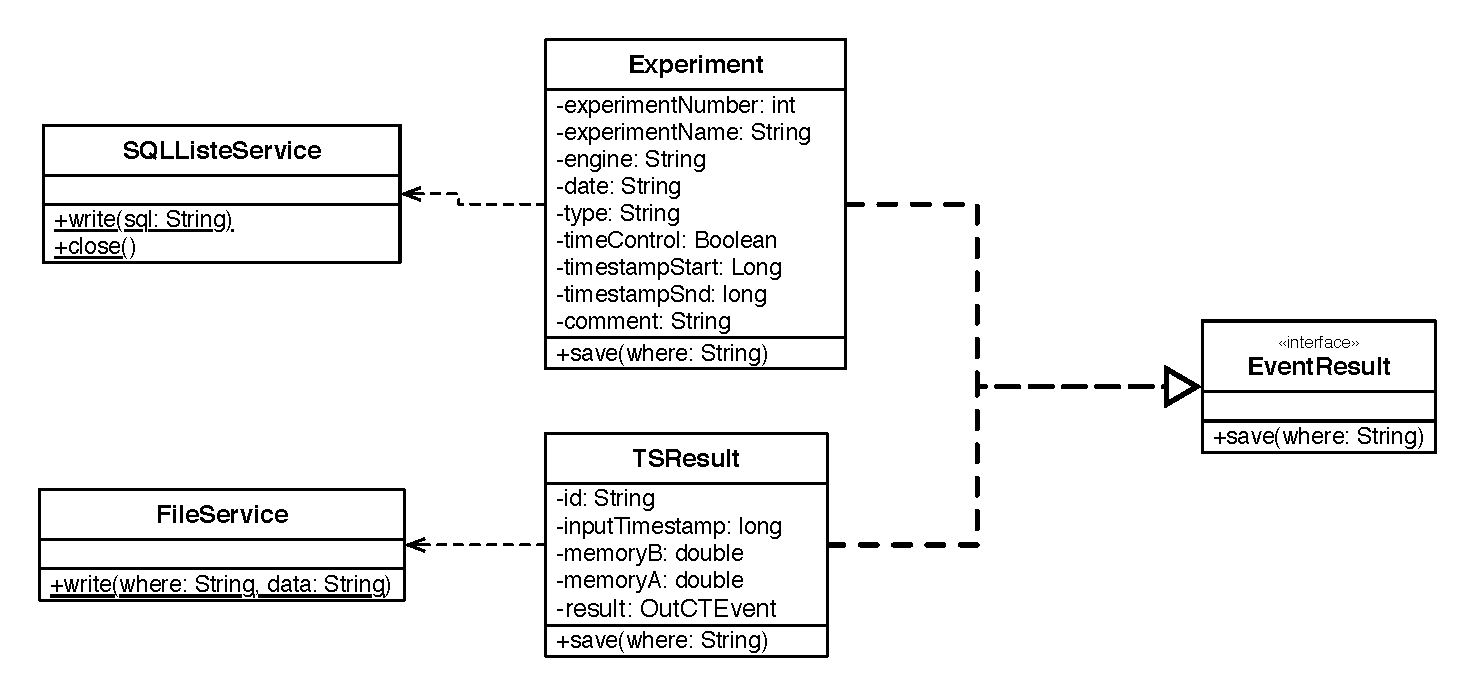
\includegraphics[width=\linewidth]{images/uml_resultcollector_events}
	\caption[\textsc{ResultCollector} Events - UML Schema]{ All the \textit{Experiment}, the \textit{TSResult} and the \textit{OutCTEvent} implements the \textit{EventResult} interface in order to hides specific saving procedure behind the \textit{save(String where)} method. The saving procedures exploits two service classes the \textit{FileService} and the \textit{SQLLIsteService}, which avoid concurrent access to the saving procedure with static methods.} 
  	\label{fig:uml_resultcollector_events}
\end{figure}

Figure \ref{fig:uml_resultcollector_events}, shows how different events in the system exploit the \textit{EventResult} interface. In the current implementation the \textit{TSResultCollector} handles two kinds of event:
\begin{itemize}
\item \textit{TSResult} - it saves the data of the query results into a TriG\footnote{http://www.w3.org/TR/trig/} file where the graph name is the event id inside the experiment, while it saves the measurements data into a CSV\footnote{$http://en.wikipedia.org/wiki/Comma-separated_values$} file that represent the time series w.r.t events id. 
\item \textit{Experiment} - it saves the experiment metadata and the tuple \\ $<\mathcal{E},\mathcal{D},\mathcal{T},\mathcal{Q}>$ collapsed into a generic description field into SQLite\footnote{https://sqlite.org/} database.
\end{itemize} 

Both the saving procedure exploit a service class, respectively the \textit{FileService} and the \textit{SQLLIsteService}. In Figure \ref{fig:uml_resultcollector_events} are describe those services, which exposes static methods to interact with the file-system. The goal is reducing system complexity offering a single point of interaction with the file-system. In this way is possible  to avoid parallel interactions that may influence the experiment. 


\subsection{Test Stand Supporting Structure}\label{sec:teststand-impl}


\begin{figure}[tbh]
  \centering
	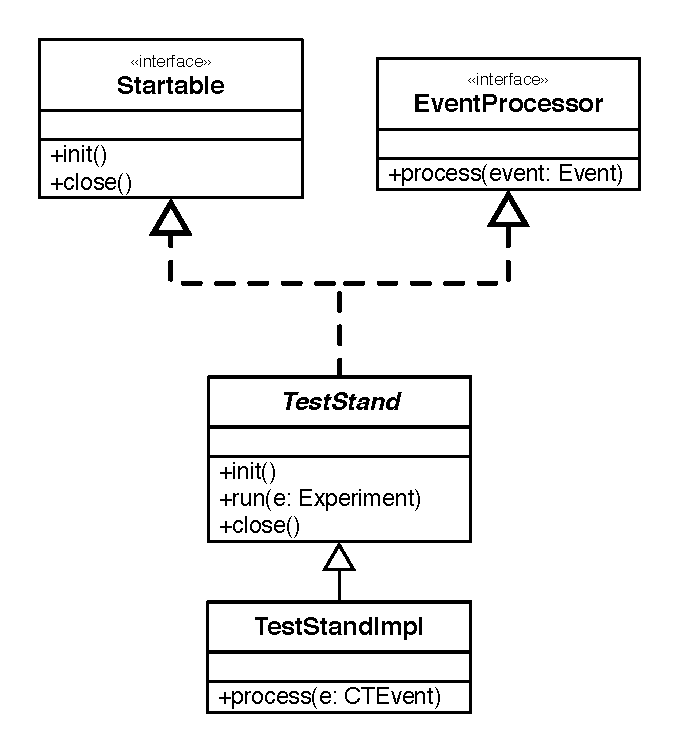
\includegraphics[width=0.5\linewidth]{images/uml_teststand}
	\caption[\name \textsc{TestStand} - UML Schema]{The \textsc{TestStand} abstract class implements both the \textit{EventProcessor} and the \textit{Startable} interfaces, but defines only the methods \textit{init()} and \textit{close()}  and it adds the \textit{run(Experiment e)} method, which encapsulate the execution logic. The \textit{process(CTEvent e)} method is implemented by \textit{TestStandImpl} which represents the \textit{Test Stand External Structure}. It orchestrates the communication between other modules and gather the data.}
  	\label{fig:uml_teststand}
\end{figure}


\noindent \name \textsc{Test Stand} was defined as set of modules which interact exchanging events during the execution. However, Chapter \ref{chap:heaven} describes at the design level the presence of an external structure which orchestrates the communication between the \textsc{Streamer}, the \textsc{RSP Engine} and the \textsc{ResultCollector}. This external structure also exposes the APIs for users interaction. Figure \ref{fig:uml_teststand} represent this idea into an UML schema where the abstract class \textit{TestStand} implements both the \textit{Startable} interface  defining the \textit{init()} and \textit{close()} methods and also the \textit{EventProcessor} interface, but it leaves the implementation of the \textit{process(CTEvent e)} method to the current implementation: the \textit{TestStandImpl}. 

The relation between the \textit{TestStand} and other modules is presented in Figure \ref{fig:uml_teststand_modules}. The \textit{TSStreamer}, the \textit{RSPEngine} and the \textit{TSResulCollector} are linked to the \textit{TestStandImpl} trough an initialisation class which receives the configuration file, and sets up these modules according with the requirements [R.1]  [R.2] and [R.3] (respectively data independence, engine independence and query independence). Once the set-up phase is completed the \textit{TestStandImpl} is initialized and it consequently initialises all the upstanding modules. The \textit{Experiment} is created externally and  the \textit{TestStandImpl} receives it to start the execution. 

\begin{figure}[tbh]
  \centering
	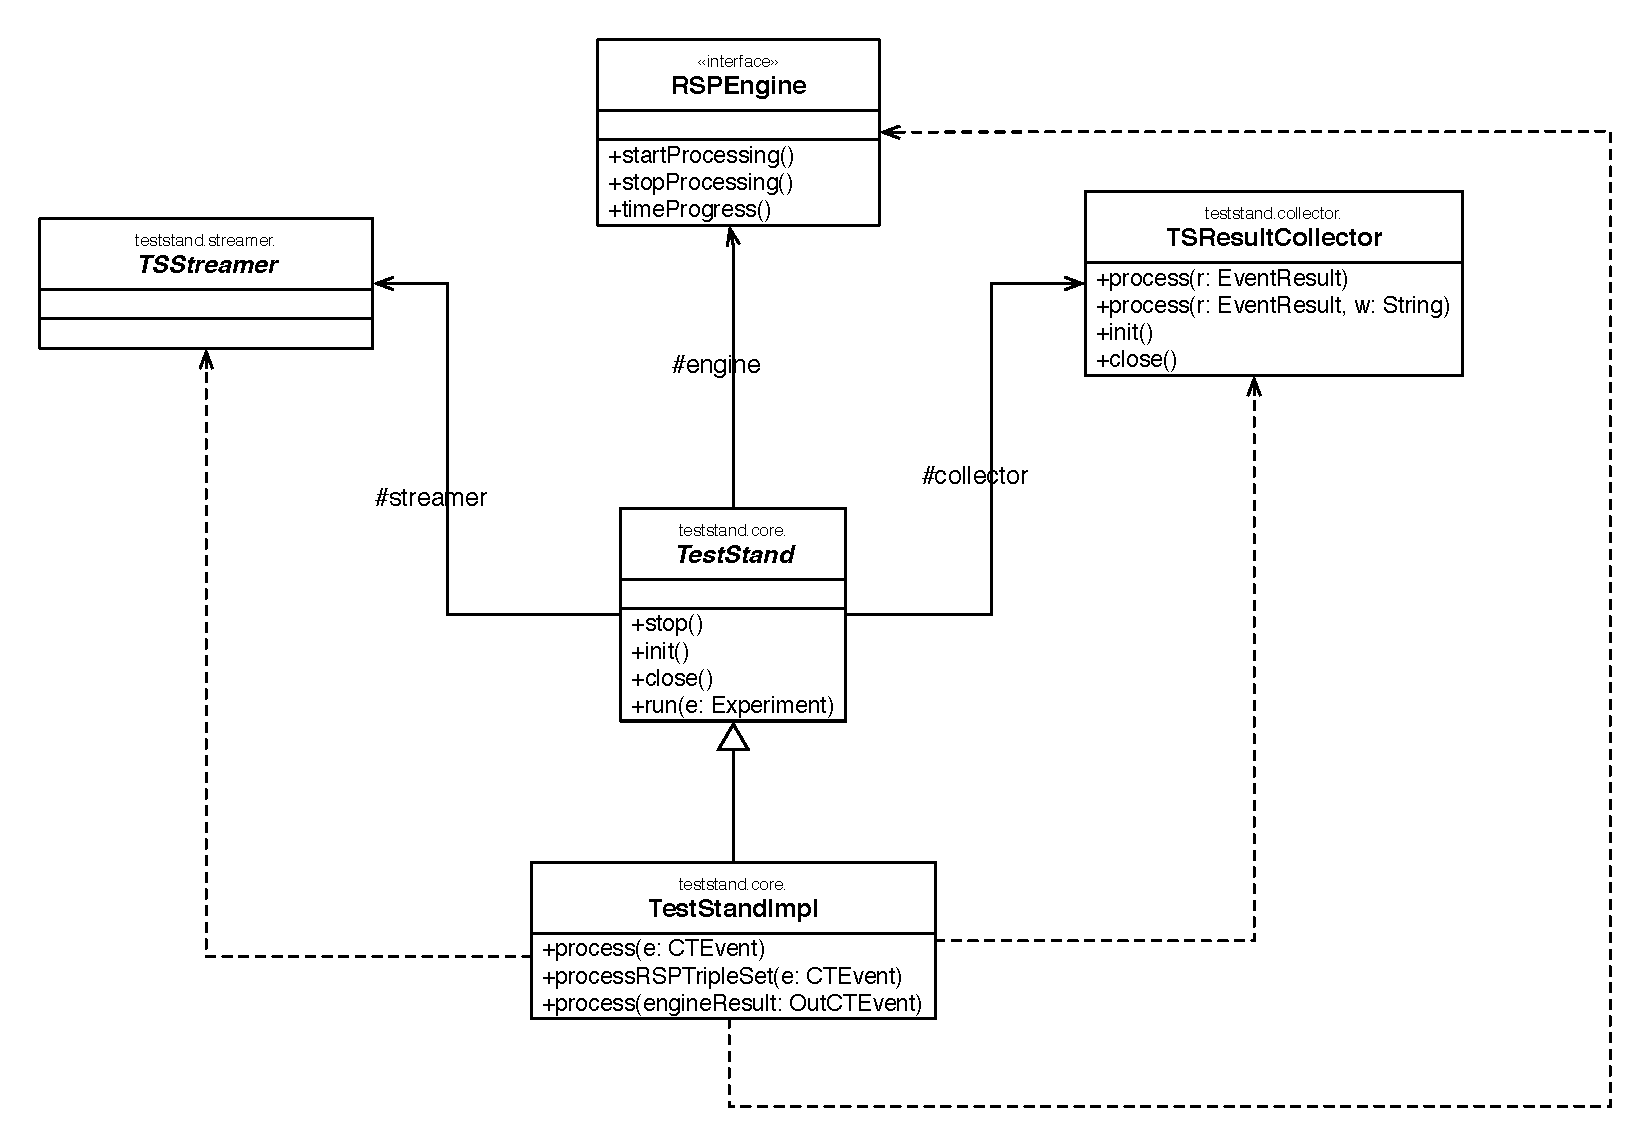
\includegraphics[width=0.90\linewidth]{images/uml_teststand_modules}
	\caption[\name \textsc{TestStand} and Modules  - UML Schema] { The \textit{TestStand} contains a reference to the modules which compose the various phases of the execution: the \textit{TSStreamer}, the engine behind the \textit{RSPEngine} interface and the \textit{TSResultCollector}. Both the \textit{TSStreamer}, and current \textit{RSPEngine} are linked to the next element in the pipeline trough the \textit{TestStand} class. Two arrows labelled with "next"  point to the  \textit{TestStand} to indicate that it is receives the events from all the other modules and orchestrates the communication. Notice that the arrow which start from the \textit{RSPEngine} is coloured in gray since is it can not be seen at this level of detail, because \textit{RSPEngine} is an interface.  the \textit{ResultCollector} receives the result to save at the end of each cycle, it does need to be linked to other modules since the process ends when it return the call.} 
  	\label{fig:uml_teststand_modules}
\end{figure}

During the execution \textit{TestStandImpl} gets the \textit{CTEvents} form the \textit{TSStreamer} and sends them to the \textit{RSPEngine} as described in Section \ref{sec:test-stand-workflow}. The \textit{TestStandImpl} gather the measurements data according with the \textit{Experiment} specification. It calculates latency starting a timer when the \textit{CTEvent} arrives and stops the timer when it \textit{RSPEngine} outputs the results as \textit{OutCTEvent}. It retrieves the memory usage asking the JVM in both the point above [R.6]. To fulfil requirements [R.7] any new measurement can take place only when the \textit{RSPEngine} is not running or when it has finished the computation. Once the \textit{OutCTEvents} comes form the \textit{RSPEngine}, the \textit{TestStandImpl} receives and immediately wraps the event into a \textit{TSResult}, which is sent to the \textit{TSResultCollector} to collect the query results data and the measurement ones fulfilling [R.8] and supporting [R.9] for further analysis with the \textsc{Analyser}.
%
%R.6 include basic set of performance measurements [?].
%R.7 enable users extensions with new software sensors and specific measure-
%ments collection.
%R.8 support performance measurements collection for further analysis.

\section{Baselines}\label{sec:baselines-impl}

\name Baselines are four elementary implementations of an RSP Engine, which  cover the requirements form [R.13] to [R.16] and implement the pipeline of a DSMS with a reasoner following the proposal presented in Section \ref{sec:baselines}. 
The RSP Engine pipeline is composed by Esper\footnote{$http://www.espertech.com/esper/$}, a mature commercial DSMS, with the Jena general purpose rule engine\footnote{http://jena.apache.org/documentation/inference/\#rules}, a flexible reasoning engine.  The aim of the choice of Esper and Jena is fulfilling requirement [R.14], baselines Eligibility by coupling two mature solutions for stream processing and reasoning to obtain a fair solution in the SR context.

\begin{figure}[tbh]
  \centering
	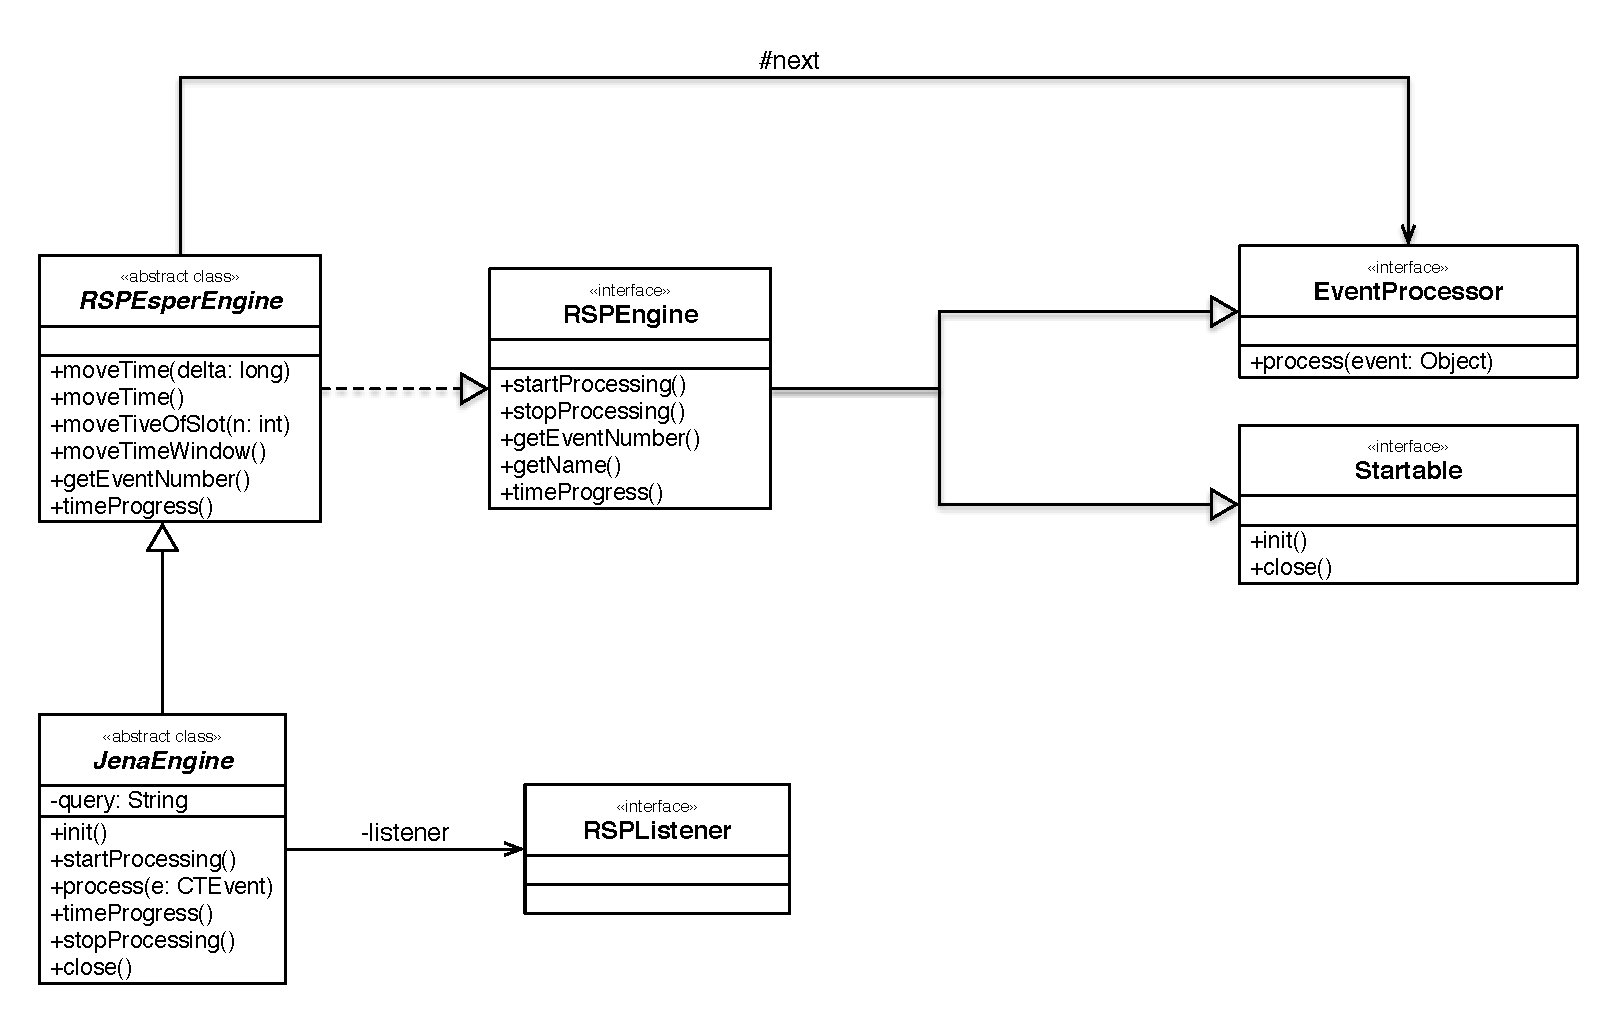
\includegraphics[width=\linewidth]{images/uml_baselines_general}
	\caption[\textit{RSPEngine} Implementation Trough Esper and Jena - UML Schema]{The \textit{RSPEngine} interface extends both the \textit{EventProcessor} and the \textit{Startable} ones. The \textit{RSPEsperEngine} class in picture implements the interface adding the Esper runtime to handle its internal events. The \textit{JenaEngine} together with the \textit{RSPListener} integrate the Jena reasoning system into the engine.}
  	\label{fig:uml_baselines_general}
\end{figure}

\noindent Figure \ref{fig:uml_baselines_general} presents how the baselines are implemented. The general structure exploits the \textit{RSPEngine} interface, a proxy for both the \textit{EventProcessor} and the \textit{Startable} interfaces described in Section \ref{sec:impl-intro} and in Section \ref{sec:modules-impl}. 

\name Baselines integrate Esper as the DSMS which compose the first half to the RSP Engine pipeline.  The \textit{RSPEsperEngine} abstract class implements the \textit{RSPEngine} interface in order to share the Esper runtime definition for all the Baselines.  They exploit the ability of Esper to be temporally controlled by an external agent\footnote{\url{http://esper.sourceforge.net/esper-0.7.5/doc/reference/en/html_single/index.html#api-controlling-time}}. Thus, the internal time flow can be synchronised by sending time-keeping events. In this way it possible to ensure the complete and soundness of query results, even in case of high traffic load. To enable external time control the \textit{RSPEngine} interface exposes the \textit{moveTime()} method.  The \textit{RSPEsperEngine} implements \textit{moveTime()} encapsulating the logic to send a time-keeping event into Esper: one time-keeping event is sent before injecting the triples within a \textsc{CTEvent} and the next one after all triples in \textsc{CTEvent} were sent. In this way all the triples in the \textsc{CTEvent} are consider contemporary by the Baselines. 

The RSP Engine is in the middle of the \textsc{Test Stand} pipeline, thus is has to communicate with the module below. The \textit{RSPEsperEngine} has a reference to a general \textit{EventProcessor}, represented in Figure \ref{fig:uml_baselines_general}  by the arrow labeled as "next", which can be any modules which processes \textit{CTEvent}. In the current implementation the \textsc{Test Stand External Structure}, implemented as the \textit{TestStandImpl} class, follows \textit{RSP Engine}, to intercept the outcoming\textit{OUTCTEvents}.

\begin{figure}[tbh]
  \centering
	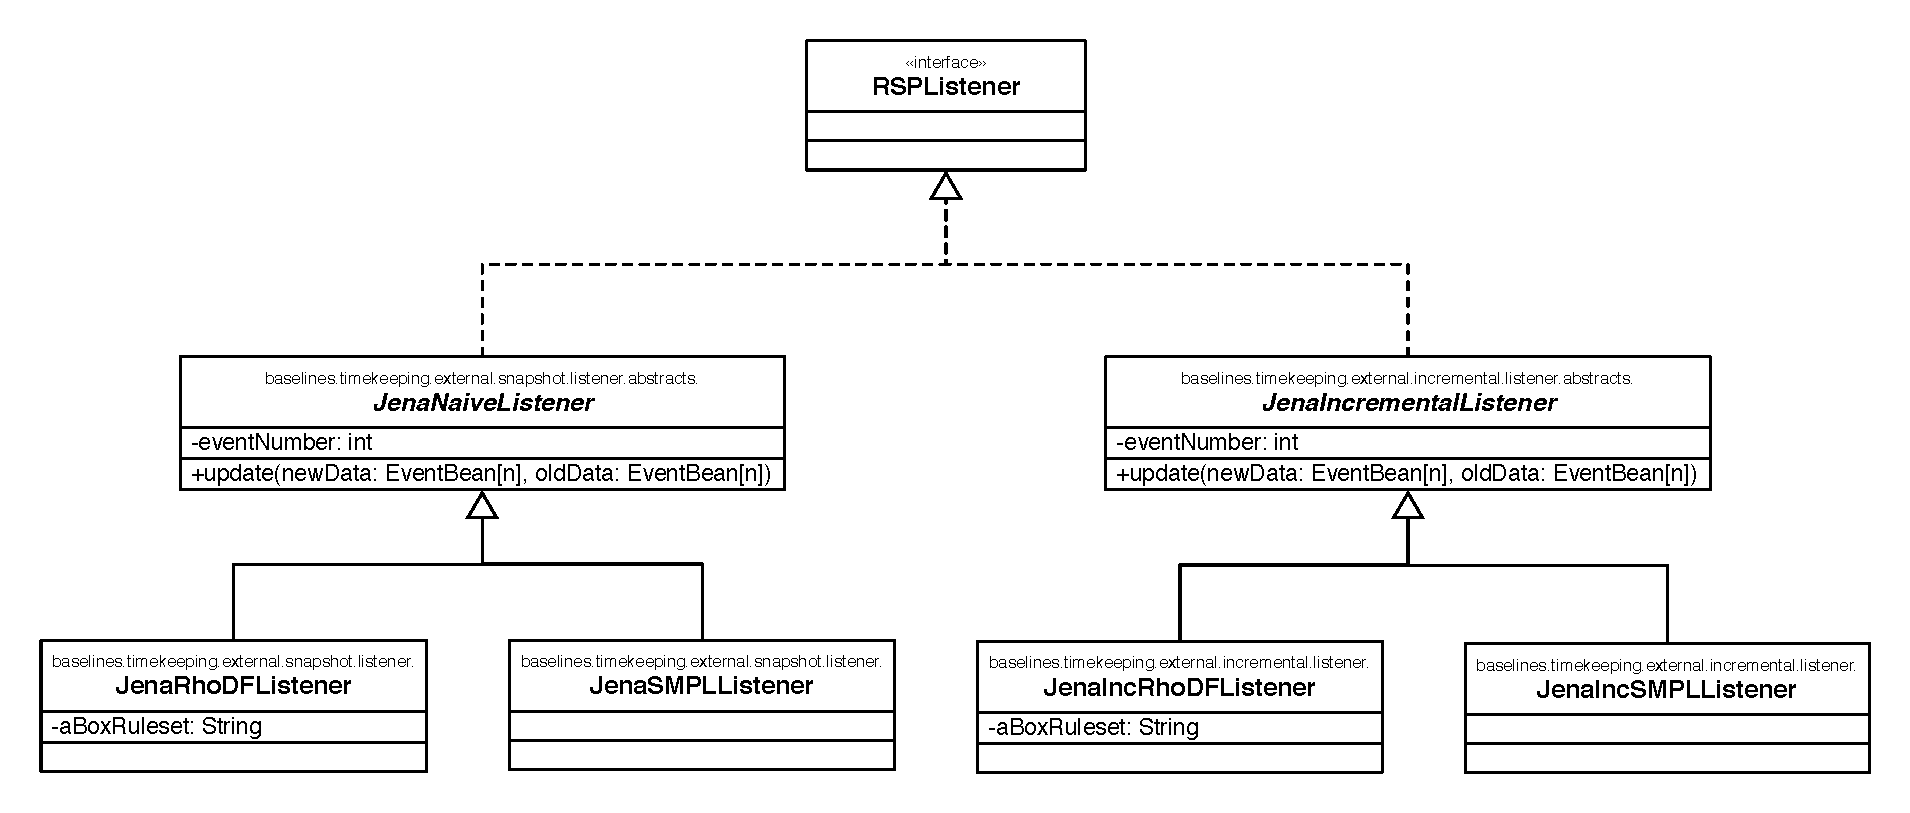
\includegraphics[width=\linewidth]{images/uml_baselines_listener}
	\caption[\textit{RSPListener} Implementations - UML Schema]{The \textit{RSPListener} is actually a proxy for the native Esper \textit{UpdateListener}. We implement the interface following two possible reasoning approaches, Naive and Incremental, respectively into the  \textit{JenaNaiveListener} and the \textit{JenaIncrementalListener}. Further implementations like the \textit{JenaNaive$\rho$DFListener} allows to specify the entailment regime and the TBox to the listeners.} 
  	\label{fig:uml_baselines_listener}
\end{figure}

We draw in Figure \ref{fig:uml_baselines_general} the UML schema of the Baseline implementation. The \textit{JenaEngine} abstract link the DSMS to the reasoner, an thus it requires a further component, the RSPListener, to complete the RSP Engine pipeline and realise the system we describe in Section \ref{sec:baselines}
 
The reasoner stage is realised as shown in Figure \ref{fig:uml_baselines_listener}. Different implementations of the listener, which all belongs to the the \textit{RSPListener} interface, variate the reasoning approaches between Naive or Incremental. The \textit{JenaNaiveListener} or the \textit{JenaIncrementalListener} partially fulfil requirement [R.15] (baseline relevance) in terms of reasoning. None of the two specify the entailment regime and the TBox, which must be defined with specific implementations like the \textit{JenaRHODFNaiveListener}, as it is visible again in the Figure \ref{fig:uml_baselines_listener}.

\begin{figure}[tbh]
  \centering
	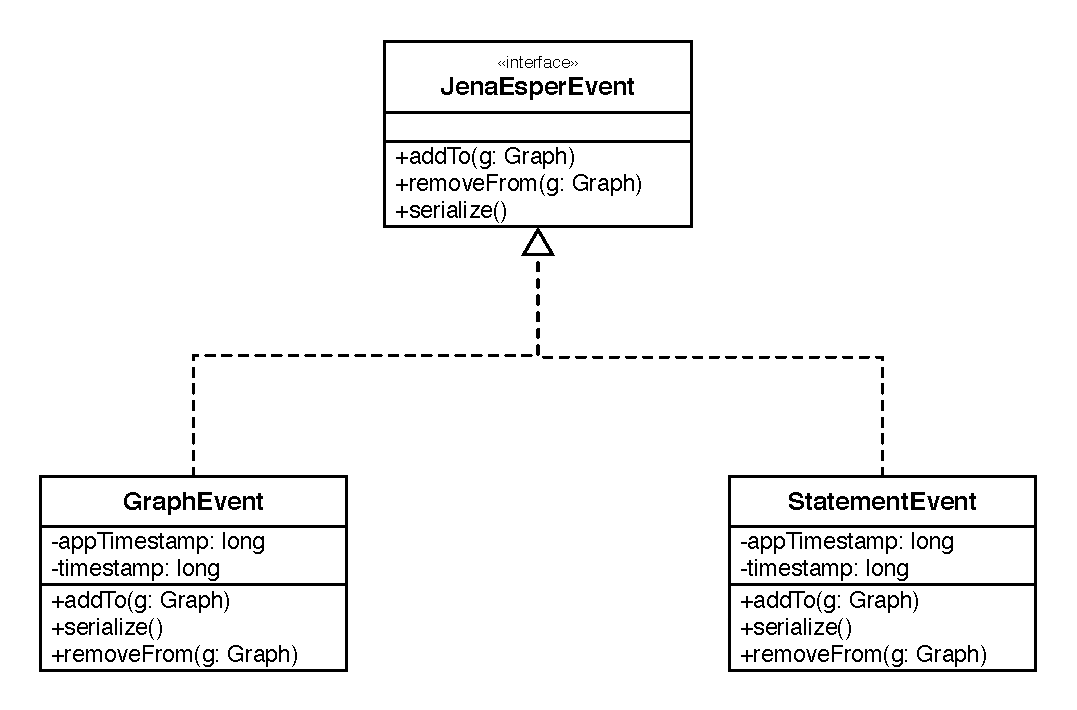
\includegraphics[width=0.7\linewidth]{images/uml_baselines_events}
	\caption[Esper-level Graph based and Triple based - UML Schema]{ All the event registered to Esper belong to the \textit{JenaEsperEvent} interface, which exposes methods to handle the reasoning independently from the RDF Stream implementation:  \textit{GraphEvent} or \textit{TripleEvent}. The triples received by the \textit{RSPEngine} can be pushed into Esper as complete graph or as a set statements. To handle the active window graph independently from the event implementation, the interface exposes the method \textit{addTo(Graph g)} and \textit{removeFrom(Graph g)}, while the \textit{serialise()} methods unroll the current event into a set of statement, in order to build an outgoing \textit{OutCTEvent}}
  	\label{fig:uml_baselines_events}
\end{figure}

The Baselines relevance demanded by [R.15] it is only partially fulfilled by the alternative reasoning approaches. It comes also from the different implementation of the RDFStream model, graph based or triple based. Esper runtime demands to registers the events that it has to handle. Figure \ref{fig:uml_baselines_events} shows how events are implemented: they belongs to the e \textit{JenaEsperEvent} interface, which exposes three methods used by the \textit{RSPListener} to manage the active window independently from event implementation. The methods \textit{addTo(Graph g)} and \textit{removeFrom(Graph g)} adelegates to the event the operations of insert and deletion to the event, in a transparent way for the \textit{RSPListener}; the method \textit{serialise()} unrolls the event into a set of statements, in this way the RSP Engine can output an \textit{OutCTEvent} independently from the RDF Stream implementation: \textit{GraphEvent} or \textit{TripleEvent}

Notice that when a \textit{CTEvents} comes to the RSP Engine it will be transformed into the events handled by the DSMS, contained in Figure \ref{fig:uml_baselines_events}. This translation process influences the latency calculus, because the time spent by the engine to translate events from the RDFStream into its internal mechanism may be relevant. Once the processing is complete, the output of the RSP Engine is translated again into an \textit{OutCTEvent} and passed to the next \textit{EventProcessor}, again spending time that influence the latency.

The current implementation of the Baselines allows to share the majority of the code by splitting the different architectural elements. In this way we fulfil [R.16] which demands baseline Simplicity, delegating to each element a specific task.

%\begin{figure}[tbh]
%  \centering
%	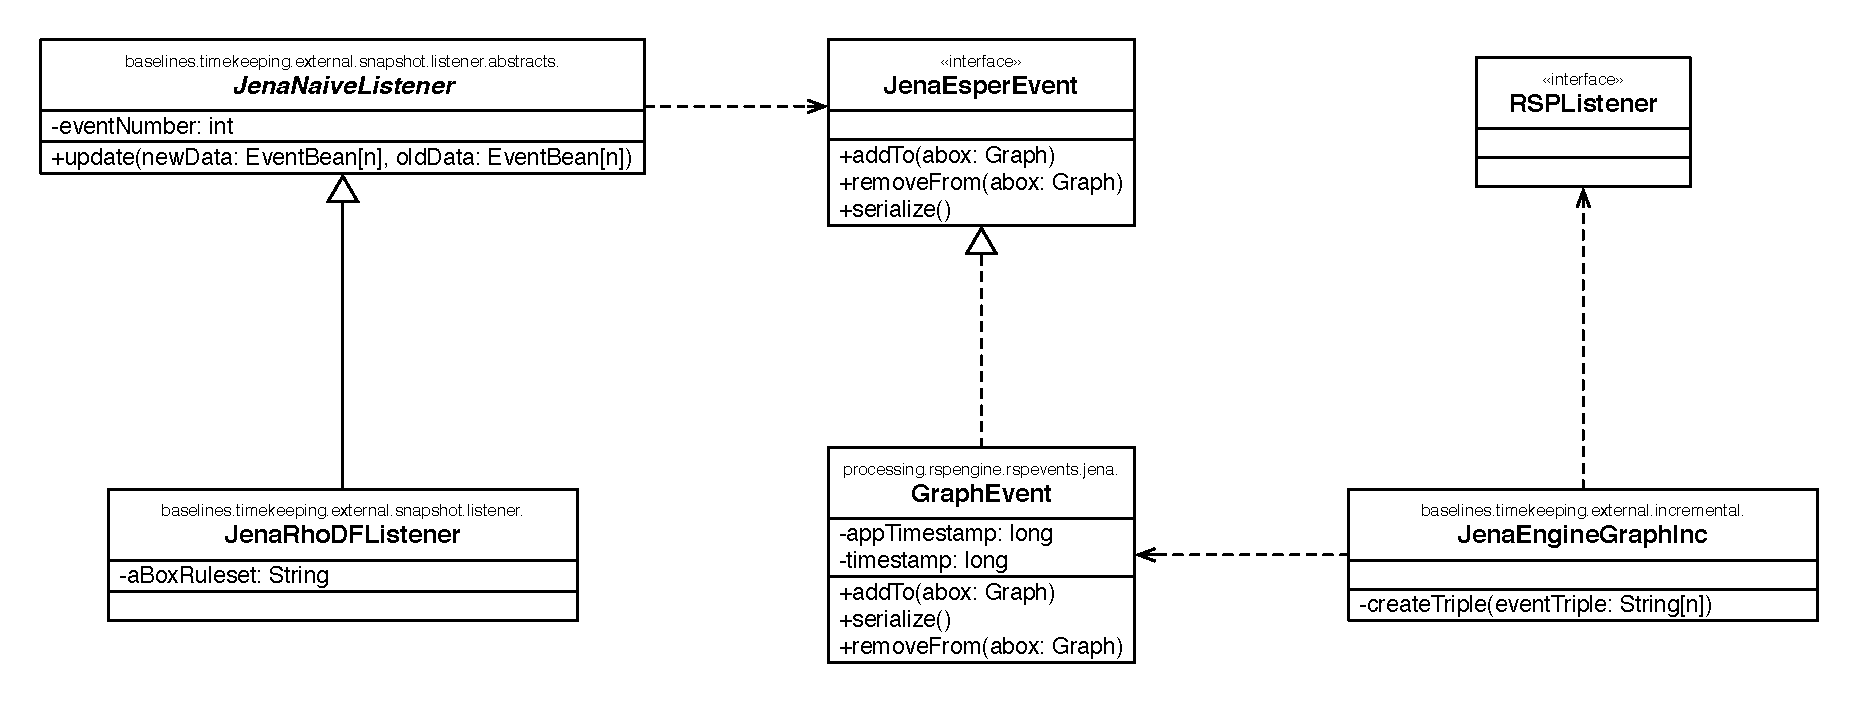
\includegraphics[width=\linewidth]{images/uml_baselines_rel_listener_event}
%	\caption[The Relation between \textit{RSPListener} and \textit{JenaEsperEvent} - UML Schema]{The listener and the event implementation are fully decoupled but logically related. In picture is detailed this relation for different implementation of the \textit{RSPListener}}
%  	\label{fig:uml_baselines_rel_listener_event}
%\end{figure}
%
%\textit{\textit{JenaNaiveListener} and the  \textit{JenaIncrementalListener} handle the events which come form the DSMS trough the \textit{JenaEsperEvent} interface, Figure \ref{fig:uml_baselines_rel_listener_event} report  the structure for the case of Graph-based event representation (see Section \ref{sec:baselines} for event details). }




\section{Analyser}\label{sec:analyser-impl}

\begin{figure}[tbh]
  \centering
	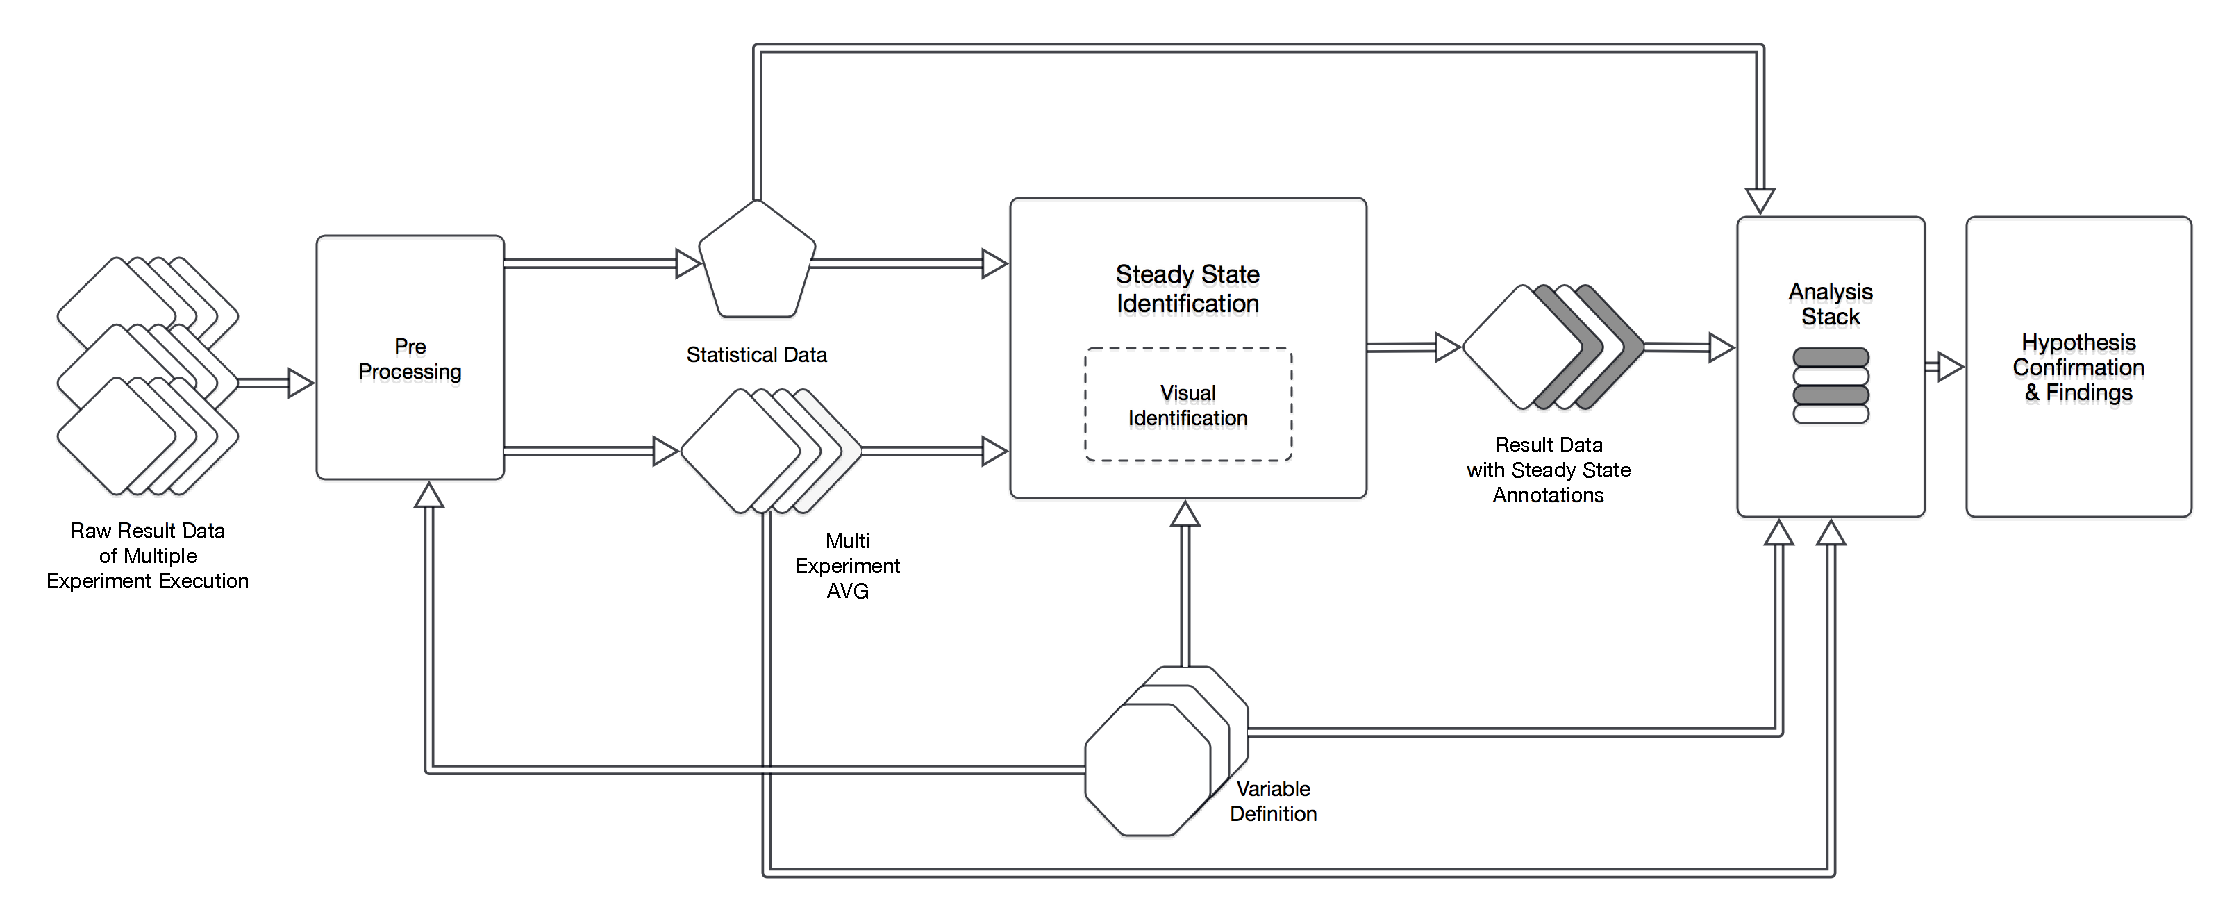
\includegraphics[width=\linewidth]{images/analyser-block-schema-impl}
	\caption[\textsc{Analyser} Block Schema: Implementation Detail Level]{\textsc{Analyser} Block Schema: Implementation Detail Level}
  	\label{fig:analyser-block-schema-impl}
\end{figure}

\noindent In this section we introduce which analysis tools sustain the each level in the investigation stack described in Section \ref{sec:analyser} and how their realized in the current implementation of \name. Notice that the relation between the hypothesis and the tools that sustain the analysis is deep, thus it is hard to generalise the investigation toolset. Hypothesis depends on the the research question, while the tools are related to the nature of the data, which again concern the experiment.  However, there are some general meaningful characteristics, which are independent from both the hypothesis and experiment, that allow us to develop a basic toolset which sustains the entire investigation stack presented in Section \ref{sec:analyser}.

Figure \ref{fig:analyser-block-schema-impl}, shows the different phases of data processing. It refers to the original block schema of drawn in Chapter \ref{chap:heaven}, but Figure \ref{fig:analyser-block-schema-impl} goes beyond the design level, providing some implementation details. 

The Figure \ref{fig:analyser-block-schema-impl} shows the \textsc{Analyser} receives two input:
\begin{itemize}
\item the raw data form the experiments
\item the variables to build the analysis
\end{itemize}


In the original block schema (See Figure \ref{fig:analyser-block-schema}) both inputs directly enter the \textit{Steady State Identification} Block (SSI) and the \textit{Analysis} Block (AB). In Figure \ref{fig:analyser-block-schema-impl}   instead, the first block in the process is the \textit{Pre-Processing Block}. Empirical analysis can not rely on a single execution of an experiment, because even if the \textit{Test Stand} is designed to be system independent, it remains a dynamic system. Thus, strange behaviours may happen while an experiment is running. In order to reduce and possible eliminate the outliers, multiple runs of the same experiment must be mediated obtaining the average measures The \textit{Pre-Processing} Block ensures data reliability extrapolating a unique dataset from multiple executions. Moreover, time series describes how a dynamic system evolves over time, so it is meaningful to attempt hypothesis verification trough statistical values, which always consider the the Steady State to allow the generalisation of the insights. The \textit{Pre-Processing} Block calculates most common statistical metrics as average , standard deviation and maximum or minimum for a certain variable.

%Indeed, both the Steady State Identification Block and Analysis Block require an automatic procedure, named pre-processing in Figure \ref{fig:analyser-block-schema-impl}, which averages the data of multiple executions of the same experiment and calculate the statistically relevant data. 

Once we have reliable data, the \textit{Steady State Identification} Block and the \textit{Analysis} Block receive them and start the analysis process. 

Finally, researches can read the analysis point out insight and theoretical results as the last block in the process describes.

Data mining procedures are very system-dependent. For this reason we include in Chapter \ref{chap:evaluation} about the \name Evaluation, concrete analysis examples, by testing the Baselines. The aim of Chapter \ref{chap:evaluation} is to demonstrate the value of \namens, but also we want to provide some guidelines for further evaluations.

The following subsections contains further details about the \textit{Steady State Identification} Block implementation, Subsection \ref{sec:analyser-impl-ss-block}, and about the \textit{Analyser} Block with the investigation stack, Subsection \ref{sec:analyser-impl-analysis-block}.

\subsection{Steady State Identification Block}\label{sec:analyser-impl-ss-block}

The Steady State Identification Block has the aim to  determines if a solution has reached the Steady State condition for a certain variable, as we describe in Section \ref{sec:analyser-analysis-block}. Automatic procedures to identify the State State condition exist, but they require dedicated studies which will be faced as future works. Currently, the SSI is not automated. It exploits data visualisation techniques, to identify, if and when Steady State condition is reached. Practically each variable in the system is plotted in the time domain over all the entire experiment and research can exclude  the initial warm-up phase form the data evaluation when that variables reaches a stable condition. 
We know that the graphical method is limited, because it must be applied for each system variable, and human criteria can nit be reliable in this kind of analysis as automatic procedures which exploits tested algorithms. Moreover, different variables may reach the equilibrium at different times, so it is researcher responsibility to properly identify the different condition for each variable involved.

\subsection{Analysis Block}\label{sec:analyser-impl-analysis-block}

The \textsc{Analyser} Design includes Five Analysis Levels (see Section \ref{sec:analyser} with increasing degrees of detail. The \textit{Analysis} Block hides the level where the comparative research approach is declined either to the visual analysis or statistical investigation. The graphical analysis method is more qualitative then the second one, but reading the information presented in graphical way can be preferred in those case where numerical data are not clear. On the other hand, the statistical investigation method demands more complex instruments to obtain the data, but allows to answer also elaborate questions with simpler answers. Following we present for all the Analysis level the method involved in the current implementation.

\subsubsection{Level 0 - Dashboards}\label{sec:impl-level0}

\noindent Figure \ref{fig:dashboard-example} contains an example of the possible Dashboard representations. We implement the dashboard to represent data on a bi-dimensional Cartesian space where memory and latency are the axis of the graph. This kind of representation allows to define solution dominance, w.r.t the involved variable, trough inter-experiment comparisons. Thus, we can easily state which RSP Engine, if any, is better then another one looking to a dashboard.

\begin{figure}[tbh]
  \centering
	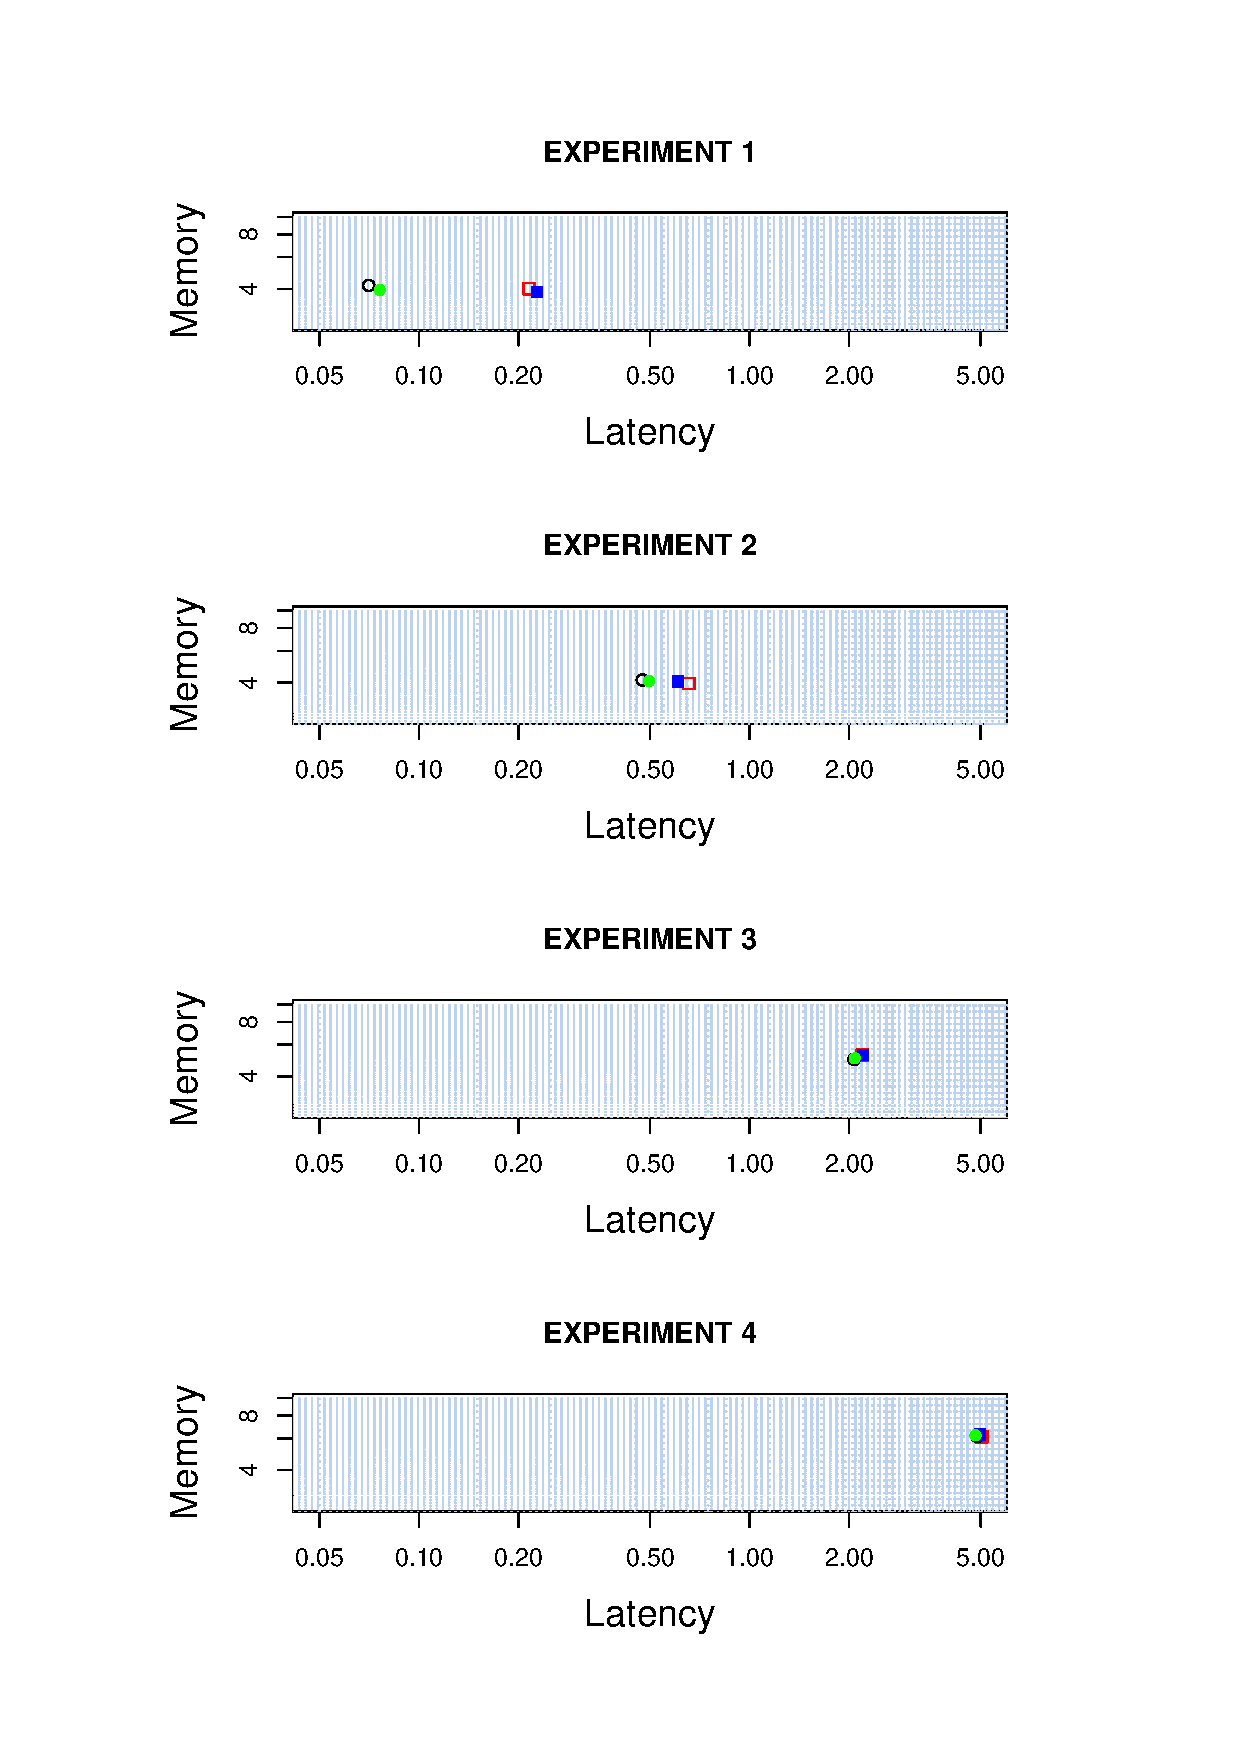
\includegraphics[width=0.45\linewidth]{images/dashboard-example}
	\caption[\textsc{Analyser} Investigation Stack - Level 0 -  Dashboard Representation Examples]{\textsc{Analyser} Investigation Stack - Level 0 -  Dashboard Representation Examples}
  	\label{fig:dashboard-example}
\end{figure}


\subsubsection{Level 1 - Statistical Values Comparison}\label{sec:impl-level1}

\begin{table}[htb]
\scriptsize
	\centering
	\subtable[Symbolic Comparison of variables A vs B on Experiment 1]{%
		\begin{tabular}{c | cccc} % creating eight columns
	  	\hline
		A vs B & \multicolumn{4}{c}{Experiment 1 Condition A}  \\
		 Comparison  & &&&\\
		\hline
		   	        & $\simeq$\\
		 Experiment 1 & A     & 	$\simeq$  & A & B\\
		 Condition  & A     & 	$\simeq$  & $\simeq$ & B\\
		 B          & A     & 	$\simeq$  & B & A\\
		\hline % inserts single-line
	 \end{tabular}
	}\qquad\qquad
	\subtable[Symbolic Comparison of variables A vs B on Experiment 1]{%
		\begin{tabular}{c | cccc} % creating eight columns
	  	\hline
		A vs B & \multicolumn{4}{c}{Experiment 1 Condition A}  \\
		 Comparison  & &&&\\
		\hline
		   	        & $\simeq$\\
		 Experiment 1 & 10\%     & 	$\simeq$  & 42\% & 33\%\\
		 Condition  & 23\%     & 	$\simeq$  & $\simeq$ & 12\%\\
		 B          & 20\%    & 	$\simeq$  & 22\% & 22\%\\
		\hline % inserts single-line
	 \end{tabular}
	}
	\caption[\textsc{Analyser} Investigation Stack - Level 1 - Qualitative and Quantitative Comparison Examples]{(a) qualitative-comparison over two variables - (b) quantitative-comparison over a common variable }
	\label{tab:comp-tables}
\end{table}

Tables \ref{tab:comp-tables} (a) and (b) show two examples of statistical investigation. Table \ref{tab:comp-tables}.a contains the qualitative comparison of two solution over a given variable, while Table \ref{tab:comp-tables}.b offers a deeper details level, the quantitative comparison, showing how much a solution is better than the other. How to choose the proper level depends on the needs of the research.

Table layout is a key-point for Level 1 representations. Tables axes represent the variation of two different experiment properties A and B. Different experiments influence the behaviour of an RSP Engine in different ways, and Level 1 allows to point out this differences with  \textit{Inter-Experiment} comparisons. Thus, we can move on the horizontal axis of Table \ref{tab:comp-tables}.a, which means variate the Condition A, to appreciate those differences. 

Actually this kind of analysis is possible thanks to a CSV report, which contains all the meaningful statistical values for the experiments. The report can be further manipulated to obtain the table visualisation.

\subsubsection{Level 2 - Patter Identification}\label{sec:impl-level2}

%\begin{figure}[tbh]
%  \centering
%   \subfigure[Pattern Recognition Example: Memory in Time Domain]{
%  	\includegraphics[width=0.45\linewidth]{images/pattern-example-memory}
%  }
%  \subfigure[Pattern Recognition Example: Memory Distribution]{
%  	\includegraphics[width=0.45\linewidth]{images/pattern-example-density}
%  	
%  }
%   %\subfigure[Pattern Appear On the Wall..]{\includegraphics[width=0.45\linewidth]{images/pokepattern}}
%	\caption[\textsc{Analyser} Investigation Stack - Level 2 - Pattern Recognition Examples]{Two examples of pattern recognition. Level 2 exploits  easy-to-read layouts which highlights the experiment difference to enable \textit{Inter Experiment} comparisons} 
%  	\label{fig:pattern-examples}
%\end{figure}

\begin{table}[htbp]
	\centering
	\scriptsize
	\subtable[Pattern Recognition Example: Memory Time Domain]{%
		\begin{tabular}{l | ccccc} % creating eight columns
	  	\hline
		Triple  & \multicolumn{5}{c}{Slots}  \\
		in & \multicolumn{5}{c}{Number}  \\
		Window  & 1 & 10 & 100 & 1000&10000\\
		\hline
			\hline
		1	   &\begin{minipage}{.09\textwidth}
     			 	\includegraphics[width=\linewidth]{images/mema-graph/N1}
    				 \end{minipage}\\			
		10	   & \begin{minipage}{.09\textwidth}
     			 	\includegraphics[width=\linewidth]{images/mema-graph/N2}
    				\end{minipage}
    			   & \begin{minipage}{.09\textwidth}
     			 	\includegraphics[width=\linewidth]{images/mema-graph/N6}
    				 \end{minipage}\\		
		100	   & \begin{minipage}{.09\textwidth}
     			 	\includegraphics[width=\linewidth]{images/mema-graph/N3}
    				 \end{minipage}
    			   & \begin{minipage}{.09\textwidth}
     			 	\includegraphics[width=\linewidth]{images/mema-graph/N7}
    				 \end{minipage}
    			   &	 \begin{minipage}{.09\textwidth}
     			 	\includegraphics[width=\linewidth]{images/mema-graph/N10}
    				 \end{minipage}\\	
		1000   &	 \begin{minipage}{.09\textwidth}
     			 	\includegraphics[width=\linewidth]{images/mema-graph/N4}
    				 \end{minipage}
    			   &	 \begin{minipage}{.09\textwidth}
     			 	\includegraphics[width=\linewidth]{images/mema-graph/N8}
    				 \end{minipage}
    			   &	 \begin{minipage}{.09\textwidth}
     			 	\includegraphics[width=\linewidth]{images/mema-graph/N11}
    				 \end{minipage}
    			   &	 \begin{minipage}{.09\textwidth}
     			 	\includegraphics[width=\linewidth]{images/mema-graph/N13}
    				 \end{minipage}\\
		10000  &	 \begin{minipage}{.09\textwidth}
     			 	\includegraphics[width=\linewidth]{images/mema-graph/N5}
    				 \end{minipage}
    			   &	 \begin{minipage}{.09\textwidth}
     			 	\includegraphics[width=\linewidth]{images/mema-graph/N9}
    				 \end{minipage}
    			   &	 \begin{minipage}{.09\textwidth}
     			 	\includegraphics[width=\linewidth]{images/mema-graph/N12}
    				 \end{minipage}
    			   &	 \begin{minipage}{.09\textwidth}
     			 	\includegraphics[width=\linewidth]{images/mema-graph/N14}
    				 \end{minipage}
    			   &	 \begin{minipage}{.09\textwidth}
     			 	\includegraphics[width=\linewidth]{images/mema-graph/N15}
    				 \end{minipage}\\
		\hline % inserts single-line
	 \end{tabular}
	}
	\subtable[Pattern Recognition Example: Memory Distribution]{%
		\begin{tabular}{l | ccccc} % creating eight columns
	  	\hline
		Triple  & \multicolumn{5}{c}{Slots}  \\
		in & \multicolumn{5}{c}{Number}  \\
		Window  & 1 & 10 & 100 & 1000&10000\\
		\hline
			\hline
		1	   &\begin{minipage}{.09\textwidth}
     			 	\includegraphics[width=\linewidth]{images/mema-dens-graph/N1}
    				 \end{minipage}\\			
		10	   & \begin{minipage}{.09\textwidth}
     			 	\includegraphics[width=\linewidth]{images/mema-dens-graph/N2}
    				\end{minipage}
    			   & \begin{minipage}{.09\textwidth}
     			 	\includegraphics[width=\linewidth]{images/mema-dens-graph/N6}
    				 \end{minipage}\\		
		100	   & \begin{minipage}{.09\textwidth}
     			 	\includegraphics[width=\linewidth]{images/mema-dens-graph/N3}
    				 \end{minipage}
    			   & \begin{minipage}{.09\textwidth}
     			 	\includegraphics[width=\linewidth]{images/mema-dens-graph/N7}
    				 \end{minipage}
    			   &	 \begin{minipage}{.09\textwidth}
     			 	\includegraphics[width=\linewidth]{images/mema-dens-graph/N10}
    				 \end{minipage}\\	
		1000   &	 \begin{minipage}{.09\textwidth}
     			 	\includegraphics[width=\linewidth]{images/mema-dens-graph/N4}
    				 \end{minipage}
    			   &	 \begin{minipage}{.09\textwidth}
     			 	\includegraphics[width=\linewidth]{images/mema-dens-graph/N8}
    				 \end{minipage}
    			   &	 \begin{minipage}{.09\textwidth}
     			 	\includegraphics[width=\linewidth]{images/mema-dens-graph/N11}
    				 \end{minipage}
    			   &	 \begin{minipage}{.09\textwidth}
     			 	\includegraphics[width=\linewidth]{images/mema-dens-graph/N13}
    				 \end{minipage}\\
		10000  &	 \begin{minipage}{.09\textwidth}
     			 	\includegraphics[width=\linewidth]{images/mema-dens-graph/N5}
    				 \end{minipage}
    			   &	 \begin{minipage}{.09\textwidth}
     			 	\includegraphics[width=\linewidth]{images/mema-dens-graph/N9}
    				 \end{minipage}
    			   &	 \begin{minipage}{.09\textwidth}
     			 	\includegraphics[width=\linewidth]{images/mema-dens-graph/N12}
    				 \end{minipage}
    			   &	 \begin{minipage}{.09\textwidth}
     			 	\includegraphics[width=\linewidth]{images/mema-dens-graph/N14}
    				 \end{minipage}
    			   &	 \begin{minipage}{.09\textwidth}
     			 	\includegraphics[width=\linewidth]{images/mema-dens-graph/N15}
    				 \end{minipage}\\
		\hline % inserts single-line
	 \end{tabular}
	}
	\caption[\textsc{Analyser} Investigation Stack - Level 2 - Pattern Recognition Examples]{Two examples of pattern recognition. Level 2 exploits  easy-to-read layouts which highlights the experiment difference to enable \textit{Inter Experiment} comparisons} 
	\label{tab:pattern-examples}	
\end{table}


\noindent Level 2 exploits the same experiment layout of Level 1, but it fills the tables cell with different charts for each experiment. Tables \ref{tab:pattern-examples} (a) and (b) are two examples. They report two possible memory analysis: representation in time domain (a) and representation of memory values distribution (b). The aim of this level is to identify patterns within the RSP Engine behaviour for a certain variable. For is reason it is necessary to appreciate together multiple experiments results, enabling \textit{Inter-Experiment} comparison.

Moving up and down in Table \ref{tab:pattern-examples}.b for example is possible to understand how memory distribution is influenced by changing the variable on the vertical axes. The same observation can be done moving from the left to the right or cross tables diagonals. Ordering experiment like in Table \ref{tab:pattern-examples} allows a new a global observations.

\subsubsection{Level 3 - Visual Comparison}\label{sec:impl-level3}

\begin{figure}[tbh]
  \centering
  \subfigure[Multi-Experiment Comparison]{
  			\includegraphics[width=0.80\linewidth]{images/comp-inter}
  			}
  \subfigure[Multi-Variables Comparison]{
  \includegraphics[width=0.80\linewidth]{images/comp-intra}
  }
\caption[\textsc{Analyser} Investigation Stack - Level 3 - Visual Comparison Examples]{Visual comparison: (a) an example of \textit{Inter Example} comparison shows the relation between memory usage in two experiment; (b) an example of \textit{Intra Experiment} comparison shows the latency and memory relation.}
  \label{fig:visual-comp}
\end{figure}

\noindent Finally, Level 3 focuses on single graphical visualisation. Figure \ref{fig:visual-comp} contains two examples of the possible analysis. 

The aim of Figure \ref{fig:visual-comp}.a shows a case of \textit{Inter Experiment} where the relation between the same variable over multiple experiments is highlighted.\ref{fig:visual-comp}.b reports an example of \textit{Intra Experiment} comparison, in order to understand the relation between memory and latency. A possible insight can be the evidence of different transitory phases before reaching the Steady State.
 \clearemptydoublepage
%The goal of this Chapter is to show how \name can improve the traditional top-down analysis method. Usually, researchers start from a deep comprehension of the theoretical problem  to to draw a model of the system over which is possible to formulate hypothesis. Further knowledge about  the implementation experience may support this method, however this approach is traditionally top-down. In this chapter we present an evaluation of \name Baselines (See Chapter \ref{sec:baselines}) in order to demonstrate how \name can extend the traditional hypothesis-based research towards the Systematic Comparative Research approach we introduced in Chapter \ref{chap:problem-settings}. Firstly, in section \ref{sec:experimental-setting} we describe the Experimental Setting, presenting our assumptions and two experiment sets for baselines evaluation. With the SOAK Test, in Section \ref{sec:soak-es}, we follow the traditional research method, showing its limitations with empirical results. In Section \ref{sec:step-es} we extends the research work on the baselines as an example of \name potential.

\section{Experimental Setting}
\label{sec:experimental-setting}

It is hard to formulate and prove hypothesis which are only based on he knowledge of the a model. The purpose of these tests is to show why is difficult to reach results trough this method, even for simple hypothesis, and consequently demonstrate that we need \namens .

The experimental setting of the evaluation consist in all the assumptions and the convention we have decided before starting the evaluation, in order to reach our goal. Practically, the experimental setting  consists into the definition of different tests to cover the most important variations on the tuple presented in Chapter \ref{chap:heaven}, which describes an experiment as $<\mathcal{D}, \mathcal{T},\mathcal{E}, \mathcal{Q}>$, where:
\begin{itemize}
\item $\mathcal{E}$ is the RSP Engine
\item $\mathcal{D}$ is the Dataset 
\item $\mathcal{T}$ is the Ontology
\item $\mathcal{Q}$ is the Query that $\mathcal{E}$ continuously answers.
\end{itemize}



The reason why we chose the Baselines as the RSP Engines $\mathcal{E}$ subject of our experiment is that Top-Down investigations are harder for commercial solutions like C-SPARQL Engine and CQELS. The the complexity of the architecture of these commercial solutions is high, and can not be easily faced in order formulate hypothesis of comparison. For the baselines instead this survey is possible. We have a complete model of their system and we also know many implementation details that can help during the analysis. Moreover,  in Chapter \ref{chap:problem-settings} we describe which requirements guarantee that an RSP Engine is a baselines (SERE properties): Simplicity, Elementarily, Relevance and Eligibility allow us to evaluate the baselines as a simple term of comparison for further research on Stream Reasoning systems and they clarify how to develop the investigation.
 
Section \ref{sec:baselines} shows that the four baselines differ for two characteristics: RDF Stream Model and Reasoning architecture. The Table \ref{tab:baselines-names} summarises these few but well determined differences, naming the four baselines for the evaluation:\begin{table}[htb]
\scriptsize
\centering
\begin{tabular}{c|cc} % creating eight columns
	\hline
         & Naive & Incremental\\
	\hline
	Graph        &  B1      & B2\\
	Statment   &  B3   & B4\\
	\hline % inserts single-
\end{tabular}
\caption{Configuration of the four baselines}
\label{tab:baselines-names}
\end{table}

\noindent Among these four configurations we formulate simple hypothesis, stating which approach is better then an other one within an experiment. How we realised the baselines is described in Section \ref{sec:baselines-impl}; the know-how about their internal mechanisms may help to find the motivations behind behaviours which are unpredictable form the architectural viewpoint. 

The Dataset  $\mathcal{D}$ and the Ontology $\mathcal{T}$ must be chose to ensure baselines Simplicity, as stated in Section \ref{sec:baselines}. We take $\rho$DF  \cite{DBLP:conf/esws/MunozPG07} as their entailment regime, because several works in the field \cite{DBLP:conf/semweb/UrbaniMJHB13} choose this as the minimal meaningful task for a Stream Reasoner. In particular, $\rho$DF is the RDF-S fragment that reduce complexity while preserving the normative semantics and core functionalities. 

The RDF streams  $\mathcal{D}$ used in the experiments are obtained streaming in different ways the data generated with LUBM  \cite{Guo2005} and the ontology $\mathcal{T}$ is the LUBM one\footnote{http://swat.cse.lehigh.edu/onto/univ-bench.owl}. We assume that the ontology does not change over time, therefore the materialisation of $\mathcal{T}$ is computed before starting the experiment and the RSP engine does not have to perform this task. It is worth to discuss the choice of using data from LUBM over SRbench and LSbench. The first one has data, which are not adequate for the experiments, since they do not require any reasoning. The SRbench data, on the contrary, requires reasoning, but, being real-data, do not have the possibility to be scaled up and down. This choice accomunate us to previous works on Stream Reasoning \cite{DBLP:conf/semweb/UrbaniMJHB13}. 

The data generator system, responsible to build $\mathcal{D}$ w.r.t. $\mathcal{T}$, is able to scale both in terms of dimension of the dataset and the reasoning effort. Being LUBM static data, we exploit the \textit{RDF2RDFStream} component of the test stand that takes care to adapt the data generate by LUBM to a streaming scenario. The component can be set up to obtain an RDFStream where the number of triples with the same timestamps follows a given discrete function, Section \ref{sec:streamer-impl} contains the implementation details of this particular \textsc{Streamer}. %e' veramente il timestamp quello?

The experiments in this Section are thought to show what kind of testing is possible trough \namens. We designed two kind of experiments based on the \textit{RDF2RDFStream} capabilities to control the triple distribution in the RDFStream. In order to evidence system dynamics over a particular input both the experiment typologies belong to the category of Stress Test:
\begin{itemize}
\item \textbf{SOAK}: the number of contemporary triple in the RDFStream does not change during the experiment.
\item \textbf{Step Response} the number of contemporary triple suddenly changes during the experiment, usually increasing of a degree of magnitude.
\end{itemize}
 
Finally, the queries $\mathcal{Q}$, used in the experiments, are variants of the same two basic identity queries that continuously asks for the materialisation of the current window:
\begin{enumerate}
\item[Q.1] Naive
\item[Q.2] Incremental
\end{enumerate}
 		 
Q.1 outputs the snapshot of the entire window and it is used for the Naive reasoning approach; Q.2 outputs the ir-streams and it is used for the Incremental reasoning approach. The queries differ for the size $\omega$ of the sliding window. In particular, we use windows in which $\omega$ is an integer multiple of the slide parameter $\beta$ of the window, i.e., it holds that $\omega = \beta * N$. In other words, $N$ is the number of \textsc{CTEvents} that the window contain. 

Moreover, Section \ref{sec:baselines-impl} shows how the proposed baselines take advantage of the ability of Esper to be temporally controlled by an external agent\footnote{\url{http://esper.sourceforge.net/esper-0.7.5/doc/reference/en/html_single/index.html#api-controlling-time}} by sending time-keeping events to synchronise the internal time flow. All the triples in the \textit{CTEvent} are consider contemporary by the baselines and each \textit{CTEvent} can be seen as a proxy for the timing event. Together with the \textit{RDF2RDFStream} is possible to estimate the content of the current window in terms of number of RDF Triples in any moment of the experiment.\\

Following we describe in details the content of the SOAK (Section \ref{sec:soak-es}) and the Step Response tests (Section \ref{sec:step-es}), providing a lecture key for the experiment results.

\section{Experiment Design}

Experiment design has the goal to prove one or more hypothesis, evidencing the behaviour of the system in the context that those hypothesis involves. Experiment design starts with some assumptions, for example in Section \ref{sec:experimental-setting} we explain the reasons why we chose $\rho$DF as entailment regime for our experiments. Researchers formulate hypothesis on the base of these assumption, and they design experiments to verify hypothesis validity. Figure \ref{fig:experiment-design} summarises this approach.

\begin{figure}[tbh]
  \centering
	\includegraphics[width=\linewidth]{images/experiment-design}
	\caption{Traditional Experiment design workflow} 
  	\label{fig:experiment-design}
\end{figure}


From a theoretical point of view we decide to study RSP Engine facing their nature of linear dynamic system. Experiment design also require to point out which variable are observed. We simplify the study analysing their behaviour in term of Latency and Memory, as reported in Chapter \ref{chap:heaven}, and comparing the results of the four baselines (see Table \ref{tab:baselines-names}) between many experiments.

\subsection{SOAK: Tests and Hypothesis}\label{sec:soak-es}

Soak testing show the system dynamics, stressing the subject with a constant and continuous input flow. In the Stream Reasoning context the RDFStream is controlled to have the same number of contemporary triple over time. 

All the experiments are 20000 events long, this duration ensures to reach for majority of the experiments the Steady State condition for both latency and the memory. Unlikely, is not possible to foretell how many events are required in to reach the Steady State condition for a certain variable, especially memory. Multiple attempts and empirical evaluation are the only way to set up the correct longness. All experiment are executed 10 times, and we take the average to reduce measurement error. 

\begin{table}[htb]
\centering
 \begin{tabular}{l|c| lllll}
	  	\hline
		\multicolumn{2}{c|}{  } &\multicolumn{5}{c}{Window size}  \\
		\multicolumn{2}{c|}{  } & 1 & 10 & 100 &1000 &10000\\
		\hline
		\hline
		 & 1 & 1 & 10 & 100 & 1000&10000 \\
		\textsc{CTEvent}      & 10  & 10  & 100  & 1000 & 10000  \\
		size             &100   & 100   & 1000 & 10000  \\
					&1000   & 1000 & 10000 \\
					&10000   & 10000  \\
		\hline 
	\end{tabular}
	
	 \vspace{10pt}
	\caption{The number of triples in the window during the ten SOAK tests as a function of the Window size (in terms of $N$) and of the triples in each \textsc{CTEvent}.}
	\label{tab:soaktests}
\end{table}

Table \ref{tab:soaktests} presents the fifteen SOAK tests we run for each baseline presented in Table \ref{tab:baselines-names}. The columns of the table are the different window sizes measured in terms of the values assumed by $N$.  Being $\beta=$ 100 ms., they the corresponds to window that span 100 ms., 1 sec., 10 sec. and 100 sec.. The rows are the different number of triples in each \textit{CTEvent} sent by the \textsc{RDF2RDFStream} to $\mathcal{E}$. Notably, for all of them, we checked that $\mathcal{E}$ is responsive for the whole duration of the experiment. 

\pagebreak

Following the traditional research method, we formulate two naive hypothesis based on the knowledge we have of the model. The hypothesis to verify with SOAK experiments are:
\begin{itemize}
\item \textbf{HP.1} The Incremental reasoning approach is always better then the naive one.
\item \textbf{HP.2} The Graph-based model for RDFStream is always better then the Triple-based one.
\end{itemize}

\subsection{Step Response Tests}\label{sec:step-es}

Step Response testing allow to see how the system reacts to a sudden changing in the input condition. 

SOAK tests usually show an initial warm-up phase for the system. With this set of experiments we can study how the system response changes if we move form an input condition to another one from a stable running condition instead of starting from scratch.

We design the step experiments concatenating two of the SOAK table ones, obtaining a total length of 400000 events, which means hours of execution for the system. For this reason we investigate only few configuration, all with 10  window slot size for all the four baselines. Table \ref{tab:steptests} summarises the step experiment set-up, where the step is positioned at the half of the execution, 20000 events.
\begin{table}[htb]
\centering
 \begin{tabular}{c|c|c}
	  	\hline
	  	&\multicolumn{2}{c}{CTEvent size}  \\
		Window Size & Initial Size & Final Size\\
		\hline
		\hline
		 10 & 10 & 100\\
		  10 & 100 & 1000\\
		 10 & 10 & 1000\\
		% 10 & 10 & 10000\\
		
		% 10 & 100 & 10000\\
		% 10 & 1000 & 10000\\
		\hline 
 \end{tabular}
	\vspace{10pt}
 \caption{}
\label{tab:steptests}
\end{table}

We do not formulate hypothesis for Step experiments. The purpose of this test set is to show \name capabilities and not to offers a deep understating of the baselines. However, we comment the results evidencing the finding in the sections below.

\subsection{Execution Environment}\label{sec:execution-environment}

All experiment are executed exploiting a dedicated machine, an iMac mid-2011 with 12GB RAM and 3.6 Ghz of a Intel i5 64 Bit, which run OS X 10.10.2 Yosemite,. Since \name is developed with Java 7\footnote{http://www.oracle.com/technetwork/java/javase/javase7locales-334809.html}, we use the versione 1.7.0.71 of the JVM.
The execution happens in a controlled environment, which tries to reduce the number of disturbing elements like network, graphical interface and other running processes.

\section{Evaluation Results}

The raw data results that comes of the experiment executions are in time series format, see Section \ref{sec:teststand} and in Section \ref{sec:teststand-impl} for details. Figure \ref{fig:data-processing} shows the phases which brings to the concrete analysis and the theoretic results. 

\begin{figure}[tbh]
  \centering
	\includegraphics[width=\linewidth]{images/data-processing}
	\caption{From raw data processing to results dashboards} 
  	\label{fig:data-processing}
\end{figure}

We need the Steady State identification step because dynamic system usually has an initial warm-up phase which negatively influences results and inhibit generalisation and comparisons. To properly contrasts results between $n$ different RSP Engines data must be standardized. Automatic procedures to identify the State State condition exist, but requires dedicated studies which will be faced as future works. At this moment Steady State identification exploit data visualisation and is done by the researchers.  

Once the Steady State is identified we process all the data, weighting them w.r.t. the results of the Steady State post-processing analysis and the Hypothesis. Dashboards are the higher level of analysis offered by \namens. The Steady State data are presented in a n-dimension space which involves all the variables selected during the experiment design phase. Comparing solution trough dashboards it immediate, we can easily identify which solution, if any, is better then the other ones.

Section \ref{sec:analyser-impl} shows the different level of analysis powered by \namens. We start presenting the SOAK Results exploiting the high level dashboard view: Figure \ref{fig:result_dashboard} shows how the baselines behaviour changes while changes the experimental setting. We compare the variation of the slot number in the active window, starting from 1 (tumbling) and moving to 10000, Figure \ref{fig:results_diagonal_5} shows this comparison.
What results state is that not only both the Hypothesis we have formulated in Section \ref{sec:soak-es} are not confirmed for all the experiment, but also that there is not a baseline which wins all the contrasts. This evidence states how difficult is to prove theoretical truth in complex system like RSP Engines, even for the Baselines which are simpler than the commercial solutions.

\name allows to better understand these results going deeply in the analysis. First of all we present in Tables \ref{tab:soak_latency_comparisons} and \ref{tab:soak_memory_comparisons}, which resumes in all the experiment which Baselines i better, fixing a certain property. Here we include the symbolic resuming table, but \name allow visualisation also of the numerical result, for a direct analysis

Tables \ref{tab:soak_latency_comparisons}  and \ref{tab:soak_memory_comparisons} show in a easy-to-read form the behaviour in terms of latency and memory. Some observation are possible on this data, because \name changes the way to investigate RSP Engines: now we can state some empirical truths and we can improve our models. 

The results in Table \ref{tab:soak_latency_comparisons}.c and Table \ref{tab:soak_latency_comparisons}.d when N=1, i.e., the window contains only one \textit{CTEvent},  allow to state for large events that the Naive approach is faster than the Incremental one. Instead, when \textit{CTEvent} contains only few triples, the Incremental approach is faster. This is not intuitive, because from theory we know that the incremental maintenance is more computationally expensive then materialisation for large changes \cite{DellAglio2014,DBLP:conf/cikm/RenP11,DBLP:conf/semweb/UrbaniMJHB13}.

When $N>$1, the results in Table \ref{tab:soak_latency_comparisons}.a and \ref{tab:soak_latency_comparisons}.b allow to say that using a Triple-base RDF stream is faster than Graph-based one. This is because the graph data structure may speed up reasoning when it contains multiple triple, but it does so introducing an overhead that may hinder performances when it contains few triples \cite{DBLP:conf/semweb/BalduiniVDTPC13}.   In particular, for the case $N$=1000 when the window contains 1000 triples (i.e., each \textsc{CTEvent} contains only one triple),  the Naive Triple-based approach is about 10\% faster  than the Naive Graph-based one while the Incremental Graph-based is even about 20\% faster.

Finally, the results in Table \ref{tab:soak_latency_comparisons}.c and \ref{tab:soak_latency_comparisons}.d supports the idea that when the number of changing triples in $\Delta+ \Delta-$ (Section \ref{sec:baselines}) is a small fraction of those in the window an Incremental approach is faster than the Naive one \cite{DellAglio2014,DBLP:conf/cikm/RenP11,DBLP:conf/semweb/UrbaniMJHB13}. The exception of the case $N$=1, but it can be considera limit case, where the reasoner is asked to deduce all the implicit triples implied by the only explicit triple in the window.  

While is possible to state meaningful observation over latency data, the same is not possible for memory ones. \name shows that the study of the memory can not be faced with the same methods to study latency, comparing the mean values at the Steady State condition. Table \ref{tab:soak_memory_comparisons} reports the  results for the memory usage during the experiments with the same representation we used for latency.  It is very hard to identify common behaviour in those results, and we can't confirm the what we observed in Table \ref{tab:soak_latency_comparisons}. However, trough \name is possible to lead the analysis to another level, observing the directly the memory usage in the time domain or in the frequency domain. 


\pagebreak
\begin{table}[htbp]
	\centering
	
	\subtable[Incremental]{%
		\begin{tabular}{l | ccccc} % creating eight columns
	  	\hline
		Triple in & \multicolumn{5}{c}{Number of Slots}  \\
		 Window  & 1 & 10 & 100 & 1000&10000 \\
		\hline
		1  	 & $\simeq$\\
		10   & Graph     &  	$\simeq$  \\
		100  & Graph     & 	$\simeq$  & $\simeq$\\
		1000 & Graph     & 	$\simeq$  & Triple & Triple\\
		10000 & Graph     & Triple  & Triple & Triple&Triple\\
		\hline % inserts single-line
	 \end{tabular}
	}\qquad\qquad
	\subtable[Naive]{%
		\begin{tabular}{l | ccccc} % creating eight columns
	  	\hline
		Triple in & \multicolumn{5}{c}{Number of Slots}  \\
		 Window  & 1 & 10 & 100 & 1000&10000 \\
		\hline
		1  	 & Graph\\
		10   & Graph     &  	Triple  \\
		100  & Graph     & 	Triple  & Triple\\
		1000 & Graph     & 	Triple  & Triple & Triple\\
		10000 &  Triple    & 	$\simeq$  & 	$\simeq$ & Triple&Triple\\
		\hline % inserts single-line
	 	\end{tabular}
	}\qquad\qquad
	\subtable[Graph]{%
		\begin{tabular}{l | ccccc} % creating eight columns
	  	\hline
		Triple in & \multicolumn{5}{c}{Number of Slots}  \\
		 Window  & 1 & 10 & 100 & 1000&10000 \\
		\hline
		1    & INC\\
		10   & INC   & INC \\
		100  & NAIVE & INC & INC\\
		1000 & NAIVE & INC & INC & INC\\
		10000 & NAIVE & INC & INC & INC& INC\\
		\hline % inserts single-line
		\end{tabular}
	}\qquad\qquad
	\subtable[Triple]{%
		\begin{tabular}{l | ccccc} % creating eight columns
	  	\hline
		Triple in & \multicolumn{5}{c}{Number of Slots}  \\
		 Window  & 1 & 10 & 100 & 1000&10000 \\
		\hline
		1    & INC\\
		10   & INC   & INC \\
		100  & NAIVE & INC & INC\\
		1000 & NAIVE & INC & INC & INC\\
		10000 & NAIVE & INC & INC & INC& INC\\
		\hline % inserts single-line
		\end{tabular}
	}	
	\caption{(a), (b) - latency results comparison between Incremental and Naive approaches; (d), (c) - results comparison between Graph-based and Triple-based models}
	\label{tab:soak_latency_comparisons}	
\end{table}
\pagebreak

\pagebreak
\begin{table}[htbp]
	\centering
	
	\subtable[Incremental]{%
		\begin{tabular}{l | ccccc} % creating eight columns
	  	\hline
		Triple in & \multicolumn{5}{c}{Number of Slots}  \\
		 Window  & 1 & 10 & 100 & 1000&10000 \\
		\hline
		1  	 & $\simeq$\\
		10   & Graph     &  	$\simeq$  \\
		100  & Triple     & 	Triple & Triple\\
		1000 & Graph     & 	Triple  & $\simeq$ & Triple\\
		10000 & $\simeq$     & Graph  & $\simeq$ & Triple&Graph\\
		\hline % inserts single-line
	 \end{tabular}
	}\qquad\qquad
	\subtable[Naive]{%
		\begin{tabular}{l | ccccc} % creating eight columns
	  	\hline
		Triple in & \multicolumn{5}{c}{Number of Slots}  \\
		 Window  & 1 & 10 & 100 & 1000&10000 \\
		\hline
		1  	 & Graph\\
		10   & Graph     &  	Graph  \\
		100  & Triple     & 	Graph  & Graph\\
		1000 & Graph     & 	Triple  & Triple & Graph\\
		10000 &  $\simeq$    & 	Graph & 	Graph & $\simeq$&Triple\\
		\hline % inserts single-line
	 	\end{tabular}
	}\qquad\qquad
	\subtable[Graph]{%
		\begin{tabular}{l | ccccc} % creating eight columns
	  	\hline
		Triple in & \multicolumn{5}{c}{Number of Slots}  \\
		 Window  & 1 & 10 & 100 & 1000&10000 \\
		\hline
		1    & INC\\
		10   & INC   & INC \\
		100  & INC & NAIVE	 & INC\\
		1000 & INC & NAIVE & NAIVE & NAIVE\\
		10000 & $\simeq$ & NAIVE & INC & INC& INC\\
		\hline % inserts single-line
		\end{tabular}
	}\qquad\qquad
	\subtable[Triple]{%
		\begin{tabular}{l | ccccc} % creating eight columns
	  	\hline
		Triple in & \multicolumn{5}{c}{Number of Slots}  \\
		 Window  & 1 & 10 & 100 & 1000&10000 \\
		\hline
		1    & INC\\
		10   & INC   & INC \\
		100  & INC & INC & INC\\
		1000 & NAIVE & NAIVE & NAIVE & NAIVE\\
		10000 & $\simeq$ &  $\simeq$ & INC & INC& NAIVE\\
		\hline % inserts single-line
		\end{tabular}
	}	
	\caption{(a), (b) - memory results comparison between Incremental and Naive approaches; (d), (c) - results comparison between Graph-based and Triple-based models}
	\label{tab:soak_memory_comparisons}	
\end{table}
\pagebreak



 \clearemptydoublepage
%In this thesis work we have presented \name -- an open source framework for empirical evaluation of RSP Engines. \name aims enabling Systematic Comparative Approach in the Stream Reasoning research field trough an RSP Engine \textsc{Test Stand}, four Baselines of RSP Engines, and an \textsc{Analyser}. 

The motivations that led this work are included in Chapter \ref{chap:problem-settings}, while in Chapter \ref{chap:heaven} we described \name design and in Chapter \ref{chap:implementation-experience} we detailed the implementation of the \textsc{Test Stand}, the four Baselines and the investigation methods which compose the \textsc{Analyser}. Finally, we provided an empirical proof of \name potential in Chapter \ref{chap:evaluation}. Within the evaluation we compared the results of two experimental sets, SOAK and Stress tests, executed on the Baselines implementations. We learnt that, even when RSP Engines are extremely simple (e.g., the baselines), it is hard to demonstrate hypothesis formulated only from a theoretical knowledge. Thus empirical evaluation is required, because results emphasised the importance of conducting comparative research based on controlled experimental conditions and, thus, the need for a open source\footnote{\url{https://github.com/streamreasoning/HeavenTeststand}} framework like \namens.

The focus on the experimental infrastructure is the main difference between \name and previous work. While SRbench and LSbench focus on RDF streams and a suite of continuous SPARQL query, \name allows to compare RSP Engines based on any RDF stream, ontology, continuous query and entailment regime. It even enables to run experiments connecting to live data streams as those used in \cite{DBLP:conf/semweb/BalduiniVDTPC13}.	

In this chapter we recap this thesis works, presenting in Section \ref{sec:research-question-conclusion} our Research Question; in Section \ref{sec:research-results-conclusion} we briefly detail \namens, our work, which issues it involved and how we answer the research question. Finally, in Section \ref{sec:research-fw-conclusion} we point out \name limitations and future works of this thesis.

\section{Systematic Comparative Research Approach of RSP Engines}\label{sec:research-question-conclusion}

Stream Processing research field is growing and the number of techniques to semantically handle data stream is increasing. RDF Stream Processing Engines, a.k.a. RSP Engines, are systems able to answer continuous extensions of SPARQL queries over RDF Streams. Due to their complexity, a systematic comparison of such systems, under repeatable conditions, is hard. 

It is worth to note that, despite the Engineering epistemology of the Computer Science works, it is still present the lack of a Systematic Comparative Research Approach (SCRA) \cite{Tichy:1995:EEC:209090.209093}. SCRA is typical of those research areas which have to face very complex systems, and have difficulty to simplify the models. Architectural analysis are useful, but they are not sufficient to evaluate RSP Engine, because their behaviour must be studied during the execution. For this reason, the Stream Reasoning community has tried to define and develop solution to evaluates RSP Engines \cite{DBLP:conf/esws/ScharrenbachUMVB13}. Recent works like \cite{Zhang2012, LePhuoc2012c, DBLP:conf/semweb/DellAglioCBCV13} supported this approach with queries, dataset and methods. However the SR community still lacks an experimental infrastructure which enables the comparison of RSP Engines independently from RDF Stream, ontology, continuous query and entailment regime.  From aerospace engineering we borrow the idea of engine test stand: a facility to develop engine trough systematic testing under precise experimental conditions. Thus, we can formulate our research question as follow:\\

\textit{”Can an engine test stand, together with queries, datasets and methods, support Systematic Comparative Research Approach for Stream Reasoning?”}

%esperiment, reproducibility, repetability and comparability to enable the SRCA by a test stand
%simple terms of comparison to support the comparative research: SERE properties
%test stand design and implmentation fulfill the requirements posed
%Analyser consist in the definition of an analysis stack which extend% the traditonal top-down investiagtion based on hypothesis formulated on the model, trough empirical findings ad different level of analysis.
%We prove the value of the empirical resarch heaven test stand enables by evaluating the baselines
%we see that even for simple system like the baselines, which model is known, upredictable results may rise
%now it is possible to improve existing RSP engine model trough finding provide by the different analysi levels of the stack

In this thesis we answered such research question presenting \name, an open source framework for SCRA of RSP Engines. In the following we provides evidence of the positive results of our work, describing each phases it involves as how they are organised in this thesis.  

In Chapter \ref{chap:problem-settings} we describe how to borrow this idea of a test stand in the Stream Reasoning research field, with the goal of RSP Engine evaluation. We exploit the traditional experiment definition to grant the rigorous and systematic test of an RSP Engine. Three main experiment properties, \textit{reproducibility}, \textit{repeatability} and \textit{comparability}, allow us to formulate the requirements that a Test Stand for RSP Engine must fulfil, in order to answer our research question. SCRA, due to its case-oriented nature, demands simple terms of comparison, namely baselines, to exploit for initial evaluation examples. In Chapter \ref{chap:problem-settings} we detail which properties a baselines must have and we formulate them as  requirements for our work.

In Chapter \ref{chap:heaven} we describe \name design. We explain how the \textsc{Test Stand} and the Baselines should be to fulfil the requirements we posed. We introduce also the idea of the \textsc{Analyser} as an investigation stack, which extends the research of RSP Engine from the traditional hypothesis based approach to the empirical and comparative one. The higher levels of the investigation stack provide a statistical evaluation of experiment results, while the lower levels focus on RSP Engine dynamics offering an overview of the engine behaviour over all the experiment execution (further details of \name implementation and \textsc{Analyser} investigation stack can be found in Chapter \ref{chap:implementation-experience}).

%Our research question asks to demonstrate if a \textsc{Test Stand} for RSP Engine can support the SCRA for Stream Reasoning. 
In Chapter \ref{chap:evaluation} we show how the traditional top-down analysis are not enough for evaluating complex systems like RSP Engines, even in case of naive implementations. Our evaluation exploits an experimental set composed by SOAK Tests and Step Response Stress Tests, executed on the Baselines implementations that we included in \name framework. The results of the analysis show how the traditional research, which formulate hypothesis only on the RSP Engine model knowledge, is still meaningful, but it can be improved trough an infrastructure like \name \textsc{Test Stand}. The evaluation conducted in Chapter \ref{chap:evaluation} has shown that it is hard to demonstrate even naive hypothesis. RSP Engine dynamics can be only partially investigated from the statistical viewpoint We need further knowledge about the RSP Engine dynamics, which means observing their behaviour at once and over the entire execution of an experiment. In this way it is possible to apply SCRA at any details level it requires.\\

\noindent \name allows to drill down the analysis over an investigation stack which covers all the aspects of the dynamic system performance analysis. Previous works have defined how to evaluate RSP Engine systems \cite{DBLP:conf/esws/ScharrenbachUMVB13} and many attempts has been proposed \cite{Zhang2012, LePhuoc2012c, DBLP:conf/semweb/DellAglioCBCV13}. 

Thus, we can positively answer   our research question, stating that \name sustains SCRA and extends the traditional top-down analysis. The proposed queries and dataset can be evaluated systematically trough \namens, It is now possible to improve existing theoretical models trough the empirical findings \name points out, which were not easily available before.


\section{Limitations And Future Works}\label{sec:research-fw-conclusion}

During \name development we faced many issues related to the heterogeneous nature of RSP application domains. These concerns limit our work in different ways. They influence \name development in term of both design and implementation. Moreover, our research of RSP Engines  is actually restricted to \name Baselines within an extremely controlled experimental setting.

The limitations on \name design and its implementation must be faced improving its models and further developing the current implementation of the \textsc{Streamer}, \textsc{ResultCollector} and the \textsc{Test Stand External Structure}. On the other hand, the restrictions on the research of RSP Engine require to exploit \name \textsc{Test Stand} in order to pursue the analysis. Finally, we consider a further possible contribution the continuation of the research of the Baselines, which has its own scientific value, as Chapter \ref{chap:evaluation} partially evidenced.

Due to these limitations, the future works and possible extensions of \name belong to the following categories:
\begin{itemize}
\item \textit{Research of RSP Engine} - it involves the empirical evaluation of RSP Engine and the comparison of benchmarking results, which are our main research interests. Thus, we plan to support our research trough \namens.
\item \textit{Software Engineering and Development} - it involves future works focuses on the different aspects of \name software, which is extendible by design.
\item \textit{Research of Baselines} - it aims to provide a complete evaluation of the Baselines as simple terms of comparison for mature RSP Engines.
\end{itemize}

\noindent We aim extending the \textit{Research Work} creating a ready-to-use benchmarking suite built upon \namens, which allows to test any RSP Engine with a set of well defined experiments. Form preliminary studies we know that to cover the most important uses case an essential set of experiment must include the following tests:
\begin{itemize}
\item[T1] SOAK
\item[T2] Stress Step
\item[T3] Stress Sine Wave
\item[T4] Random Distribution (e.g., gaussian and exponential)
\end{itemize}

The experiments definition still follows the tuple $<\mathcal{E},\mathcal{D},\mathcal{T},\mathcal{Q}>$. The ready-to-use benchmarking suite will give the user the possibility to execute those test on his own RSP Engine. Moreover it should include \name Baselines as example of $\mathcal{E}$ and simple terms of comparison for benchmarking results.

SOAK Test [T1] and Stress Step Test [T2] are already part of this thesis work in a restricted form, while the other ones are not implemented yet. 

We develop [T1] and [T2] registering to our $\mathcal{E}$ as queries $\mathcal{Q}$ variations of the identity query, which a differ for window size $\omega$, because in the current stage of development it is possible to configure only the ontology and the entailment regime of the Baselines. We intend to continue the development of the Baselines, adding the possibility to register one or more continuous queries into them and exploiting more complex entailment regime than $\rho$DF. 

We have also to define which queries $\mathcal{Q}$ to include in all the experiments, considering many works in the field \cite{DBLP:conf/esws/ScharrenbachUMVB13, Zhang2012, LePhuoc2012c, DBLP:conf/semweb/DellAglioCBCV13}.

The current experiment sets [T1] and [T2] exploit LUBM ontology as $\mathcal{T}$ and the RDF Stream $\mathcal{D}$ is generated trough a module, the \textsc{RDF2RDFStream}, which adapts LUBM data to a streaming scenario (See Chapter \ref{chap:implementation-experience}). In order to generate data for all the remaining test sets [T3] and [T4] we have to extend the \textsc{RDF2RDFStream} to generate: a random flow with a given distribution (e.g., gaussian and exponential), and a sine wave flow (to mimic the periodic changes in the flow rates observed on social media streams \cite{DBLP:conf/semweb/BalduiniVDTPC13}).

Independently from the experiment set, we indent to extend the metrics gathered by \name \textsc{Test Stand}. Quoting from \cite{DBLP:conf/esws/ScharrenbachUMVB13} the possible extensions are:
\begin{itemize}
\item Response time over all queries (Average/$1^th$ Percentile/Maximum).
\item Maximum input throughput in terms of number of data element in the input stream consumed by the system per time unit.
\item Minimum time to accuracy and the minimum time to completion for all queries.
\end{itemize}

As we stated in Chapter \ref{chap:evaluation}, the content of the current window influences the RSP Engine performances for two factors: the window size before the reasoning and after. The second metrics is relevant for the RSP Engine evaluation. When the system has to handle a big number of outgoing triples we can observe a degradation in terms of memory and latency. Thus, an evaluation of the number of inferred triples w.r.t the window content at time $t$ allows to weight the engine performance results in relation to the input RDF Stream, helping to eliminate outliers and properly evaluate RSP Engines. Moreover, this observation opens new scenarios in the Stress Testing design, where the stress factor depends on the reasoning potential of the current window w.r.t a certain entailment regime.\\

\noindent Future works on \textit{Software Engineering and Development} regard the \textsc{Analyser}.  We aim to complete automate the analysis procedure, involving at least the current measurement set and tools. 

As a long term goal, we intend to standardise and publish the entire tool-set which supports analysis methods presented in Chapter \ref{chap:heaven}. We are imagining the \name \textsc{Analyser} as a Web-based environment where all existing RSP engines are already available and those: who want to run experiments, have just to configure them picking up one or more RDF streams, ontologies, and queries; who want to compare the results of its own RSP Engine can upload the raw data and wait for the evaluations results. A visual facility to compare different experiments and the publication of result experiments as linked data would complete this environment. \\


\noindent Finally, by evaluating the Baselines to prove \name potential we identified an intrinsic scientific value of this analysis. We would like to continue the \textit{Research of Baselines}, proving another contribution beyond the developments proposed above. In order to study the problem of responsiveness we have to add four alternative implementation of the Baselines, which do not exploit the external time control. The Baselines should be evaluated by [T1] T2] [T3] and [T4] but also with real data and a $\mathcal{T}$ different from LUBM, for example exploiting LS Bench queries and data to design an experiment set. 
 \clearemptydoublepage



\include{AppendiceA} \clearemptydoublepage



\nocite{*}
\bibliographystyle{plain}
\bibliography{thesis}


\clearemptydoublepage

\listoffigures
\addcontentsline{toc}{chapter}{Elenco delle figure}%
\clearemptydoublepage

\listoftables
\addcontentsline{toc}{chapter}{Elenco delle tabelle}%
\clearemptydoublepage



\end{document}
